\documentclass[12pt, letterpaper]{article}

%% My used library
\usepackage{float}
\usepackage{subcaption}
\usepackage{booktabs}
%% My used library
\usepackage{subcaption}
\usepackage{amsmath,amssymb}
\usepackage{graphicx, adjustbox}
\usepackage{caption}
\usepackage{longtable,booktabs,array}
\usepackage{csquotes}
\usepackage{multirow} % Required for multirows
\usepackage{longtable,booktabs,array}
\usepackage{calc} % for calculating minipage widths
\graphicspath{{Figs}{Figs/}}


\title{My first LaTeX document}
\author{Hubert Farnsworth\thanks{Funded by the Overleaf team.}}
\date{August 2022}
\begin{document}
\maketitle
We have now added a title, author and date to our first \LaTeX{} document!\cite{chen2018}


In Bangladesh there is lacking in effective acquisition, synthesis skill of English language from National Curriculum and Textbook Board (NCTB) curriculum provided textbook \cite{report_schools_2018, statistics_bangladesh_2017}. Specially in the rural area in National Board examinations like SSC, HSC most of the student get poor marks in English subject \cite{noauthor_bangladesh_2021, habib_english_2018}. It is anticipated students have lacking in understanding context. Topic modeling can play a significant role for context understanding for curriculum provided English textbook \cite{qiang2020short, bethard_topic_2009, ali_transportation_2019, slater_using_2017, guerra_when_2013}. Topic modeling is machine learning technique of Natural Language Processing field, offers a promising unsupervised approach to identify latent topics within provided documents \cite{jelodar_latent_2019, gupta_pan_lda_2021, pichardo_lagunas_svd_lda_2015, selvi_classification_2019, pichardo_lagunas_svd_lda_2015_1}. It can help identify the main themes, concepts, and topics within the textbook\textquotesingle s content, enabling instructors to tailor the learning experience to individual students. LDA is one the prominent algorithm which can be used for topic modeling \cite{blei2003latent}. It provides coherent topics, dominant keywords, latent combination of features that characterizes similarities between topics. In this research LDA extracted keywords are rearranged and incorporated into a mobile app to observe user experience. 

Across all English learning applications via digital media, about 55\% exercise activities involved vocabulary learning \cite{klimova_evaluation_2018, hao_evaluative_2019, polakova_mobile_2019} and other exercises includes quizzes, flash cards, and games \cite{xu_scoping_2020, shortt_gamification_2023} for enhancing learners' comprehension and self-checks ability \cite{bernacki_mobile_2020, metruk_use_2021, isamiddinovna_mobile_2019, klimova_evaluation_2018}. Therefore, it can be assumed that if LDA extracted vocabulary is learned then it will improve contextual understanding, enhance synthesis knowledge of subtle meaning of correlated topics. There are numerous English learning apps are prevailing \cite{metruk_use_2021, rafiq_sustaining_2021, chen_evaluating_2016}. One caveat is of these apps are very few of them are based on Curriculum Board provided Textbook for learning English hence, could not able to attract a large number of pupils in Bangladesh who are mostly depended on NCBI textbook.  To grasp the English language knowledge from curriculum provided textbook a novel approach Latent Dirichlet Allocation (LDA) based unsupervised Topic modeling using textbook corpus is adopted and exploratory analysis is demonstrated in this study. Our anticipation is through this way student can able to interpret meaningful information facilitates students to understand the correlated topics and important keywords related to that topics leads to understand the subtle meaning of the textbook context.

\subsection{Research Overview} 
To detect underlying themes or topics keywords within a Textbook corpus an unsupervised probabilistic topic modeling technique LDA is used in this research \cite{jelodar_latent_2019, gupta_pan_lda_2021, pichardo_lagunas_svd_lda_2015, selvi_classification_2019, pichardo_lagunas_svd_lda_2015_1}. Topic modeling of LDA doesn\textquotesingle t directly account for student engagement such as learning tasks in mobile apps \cite{sandberg_mobile_2011}. Hence a prototype app is developed and qualitative survey is conducted to observe the instructor\textquotesingle s sentiment impact similar to research paper in \cite{oz2015investigation}. Qualitative survey research is undertaken to evaluate the effectiveness of unsupervised topic modeling LDA Bangladesh\textquotesingle s National Curriculum Textbook Board (NCTB) provided English Textbook for Higher secondary school education. This study seeks to ascertain if instructors can teach and students can learn English better if a mobile app is introduced which includes NLP\textquotesingle s LDA driven topic modeling applied extracted keywords and analysis. A prototype mobile app is developed to incorporate the topic modeling extracted keywords into the app. This article presents the key findings and insights from the survey, shedding light on the prospective of learners especially instructors. In the survey questions, it was indicated whether the students, teachers/instructors would find it acceptable and appreciated if textbook information were made available through a mobile app and presented in interactive format. To demonstrate the mobile app idea during the interrogation survey session a prototype is also prepared. Participants were asked for suggestions on how to make the app better and about any shortcomings. After collecting feedback, word clouds were used (see \ref{wordcloud}) to analyze the frequency of the participants\textquotesingle{} recommended terms, and the LIWC approach was used to estimate overall sentiment (see \ref{liwc}). The survey\textquotesingle s findings show that teachers are eager to use NLP provided extracted keywords technology in teaching and learning, and there are tremendous opportunities.

\subsection{Topic Modeling}
 Different techniques have been developed to perform topic modeling in the unsupervised topic modeling domain of Natural Language Processing (NLP), having their own strengths and limitations \cite{vayansky2020review, abdelrazek2022topic, yi2009comparative}. Apart from LDA, Mallet LDA, Structural Topic Model (STM), Hierarchical Dirichlet Process (HDP), Non-Negative Matrix Factorization (NMF), Latent Semantic Analysis (LSA) etc are also prevailing and can be considered for comparative research study.

\subsubsection{Topic models comparative analysis}
While some variations of LDA, Mallet LDA is considered for large corpus processing and analysis \cite{vayansky2020review, abdelrazek2022topic, Comparison_Topic_Modeling_Algorithms}. It focuses on scalability, If large corpus needs to analyze, Mallet LDA might be more suitable. LDA in general can still be efficiently applied to moderately sized corpora. Analyzing topics within the context of metadata, STM could be a better fit. Hierarchical Dirichlet Process (HDP) can be useful when we cannot guess the number of topics in advance. In \cite{Comparison_Topic_Modeling_Algorithms} LSI, NMF and LDA are compared in terms of coherence and similarity measures for social media dataset and in their analysis NMF is observed most effective measures. However, as a baseline model LDA is often considered one of the most prominent choices. In this study Textbook corpus is divided into lessons which is a mixture of topics and using LDA expecting to determine which word in the lesson belong to Lesson\textquotesingle s topics. LDA produces interpretative results for exploratory topic analysis. The identified topics are represented as distributions over words, making it easy to assign meaningful labels to topics. Provided by most of the libraries and tools, making it easy to implement and can be integrated into existing workflows. Hence, LDA serves as a solid baseline for topic modeling tasks.  

\section{Latent Dirichlet Allocation (LDA)}
LDA model considers documents are mixes of topic, and each topic is a distribution over words. The objective is to derive the hidden topic assignments and the topic-word distributions that most effectively describe the observed documents. The goal of LDA is to uncover these latent topics from a collection of documents without needing any prior labeling or categorization of the content. An expression for the joint distribution of the LDA model is described below:  
\begin{equation}
P(\theta_d,z,w\|\alpha,\beta)=P(\theta_d\|\alpha)\prod^N_{n=1}P(z_{d,n}\|\theta_d)P(w_{d,n}\|z_{d,n},\beta)
\end{equation}
Where $w_{d,n}$ the $n_{th}$ word in document $d$, $z_{d,n}$ the topic assigned to the $n_{th}$ word in document $d$, $\alpha,\beta$ are the Dirichlet LDA model parameters. controls per-document topic distribution, and per topic word distribution. $\theta_d$ represent the topic distribution. $P(\theta_d \| \alpha)$ Dirichlet 
distribution representing the document-topic distribution, $P(z_{d,n}\|\theta_d)$ is the word topic assignment for the $n_{th}$ word in document $d$, $P(w_{d,n}\|z_{d,n},\beta)$ is the distribution representing the observed word given a topic. We have chosen LDA for baseline statistical topic modeling tool. However, how many topics are ideal it is needed to determine and also topic modeling quality needs to measure.


\subsection{Optimal Topics with Coherence}  
Coherence score measure how coherent or interpret the words in that topic and estimates number of topic clusters. Coherence score assess the quality of the topics produced by LDA and ensures that the topics generated are statistically significant. Coherence \(C_{topic}\) can be expressed as follows  
\begin{equation}
C_{topic}=\sum^N_{i=1} (\frac{1}{N(N-1)}\sum^i_{j=1} PMI(w_i,w_j)
\end{equation}
Where, \(PMI\left( w_{i},w_{j} \right)\) represent pointwise mutual information statistical association between two words occurring together. PMI score indicates that the two words are more closely related within a topic. \(PMI\left( w_{i},w_{j} \right)\) can expressed as  
%\begin{equation}
%\(PMI\left( w_{i},w_{j} \right) = \log\frac{P\left( w_{i},w_{j} \right)}{P\left( w_{i} \right)P\left( w_{j} \right)}\)
%\end{equation}

where \(P\left( w_{i},w_{j} \right)\) is joint probability of occurrence of words \(w_{i}\) and \(w_{j}\).  To calculate the coherence score genism library provides range of options such as \(u_{mass},c_{v},c_{uci},c_{npmi}\). \(u_{mass}\) and \(c_{v}\)These two methods are most popular. For given topic with words \(\{ w_{1},w_{2},w_{3},\ldots..,w_{n}\}\) a fixed context window size is provided (default size 10 words) then coherence score is calculated using an equation \(\sum_{j = 1}^{i}{PMI}\left( w_{i},w_{j} \right)\) which provides negative coherence score. \(c_{v}\) can be expressed as  
%\begin{equation}
%\(c_{v} = \frac{1}{N(N - 1)}\sum_{j = 1}^{i}{similarity\left( w_{i},w_{j} \right)}\)
%\end{equation}
in which \(similarity\left( w_{i},w_{j} \right)\) represent the pairwise similarity between terms based on \(PMI\left( w_{i},w_{j} \right)\) scores. \(c_{v}\) provides a positive coherence score. Higher coherence values indicate that the topics are more coherent and representative of meaningful themes within the text data. Coherence score 0.5 are fairly good {[}43{]}.
  
\section{Literature Review}

LDA based topic modeling has been used for semantic search, ontology exploration, classification, dominant keywords searching in many research studies. For curriculum based textbook study it could be an option is not revealed from rigorous search in online repositories, which we addressed in this research study. This research model is infusing Textbook features into LDA based topic modeling to discover a set of topic-words from the provided document for Textbook comprehension and understanding context. Similar approaches and implications are described below:

\subsection{LDA for Textbook Content}

According to Krishna Raj \cite{raj_p_m_sentiment_2022} the human brain has a propensity to forget a number of facts regarding the events in book. The LDA model can able to scan through large quantities of text in the book and extract intriguing key concepts terms. Thereby, a book can be adapted by learners with the help of the LDA model, greatly refine the learning process. Similar approch proposed by  Rani for Hindi books and stories, a topic modeling text summarizing approach proposed in 2021 \cite{rani_extractive_2021}. By incorporating linguistic features into LDA-based topic modeling, the suggested model is can find a set of topic-words from the given material to understand context.  Educational content-based topic modeling for an Intelligent system to develop a tutoring system is proposed in \cite{slater_using_2017} by researcher Stefan Slater in 2017. To understand the linguistic content of mathematical problems, a personalized learning system is suggested that makes use of correlated topic modeling of natural language processing, an approach which can extract important keywords. A variety of significant and useful contents are explored in the context of addressing mathematical difficulties. They demonstrated that topic modeling is a useful method for a personalized learning systems. For key terms detection within articles LDA based topic modeling has been used in many research studies in which dominant keywords reveals future research trends or most prominent topics. Investigation of Julio Guerra in 2013 demonstrated how the LDA model can be utilized for online content linking for any major subject such as: elementary algebra \cite{guerra_when_2013}. It can also be used to simplify context comprehension and content modeling for collections of reference books on the same topic. They concluded that the recommendation provided by LDA topic modeling for online educational systems is promising.

\subsection{LDA for Dominant Keywords Determination}

In 2019 Wafa Shafqat \cite{shafqat2019topic} proposed an architecture model for better understanding of crowdfunding comments posted by the investors to understand their motive to classify whether comments are scam or legitimate comments. Deep neural network Language modeling either LSTM or RNN encoded embedding vectors are fed into a LDA based topic modeling model to understand the context of discussion trends. Compared to simple Neural Networks (NNs) and non LDA based approach this techniques performs better understanding crowdfunding comments. The capability of LDA-based topic modeling to detect the reseach trend of Bengali news published in web was analyzed by Kazi Masudul Alam in 2020 \cite{alam_bangla_2020}. Their research demonstrates that using an appropriate corpus and labeled LDA is an effective combination model for predicting news topics efficiently. LDA Labels key terms makes articles easier to read. Another research article of J. Lee published in 2022 conducted experiment on research trends of "COVID-19 and sports \cite{lee_lda_based_2022}. It used LDA and explored latent knowledge connectivity dimension and structures in the articles. Rahul Gupta  uses the application of LDA in 2022 to analyze research patterns of "Applied Intelligence" in 3269 articles published between 1991 to 2021 \cite{gupta_prediction_2022}. In this research BoW and TF-IDF embedding are used for LDA based topic modeling.

\subsection{LDA based Sentiment Analysis}

Sentiment analysis has been a key research area of NLP based research domain, where LDA has been applied to determine significant features and those features contributes to segregate sentiments and provide recommendations. LDA based topic modeling has been used in sentiment analysis task. In 2021 Y. Cho published research study of LDA-based topic modeling for sentiment analysis using topic/document/sentence (TDS) model \cite{farkhod_lda_based_2021}. This article proposed TDS novel approach that combines LDA-based topic modeling for sentiment analysis within documents. H. Wang and et. al examined Chinese people's public perception about Omicron variants on social media Sina Weibo. Social Media's 121,632 omicron related data post were analyzed using LDA-based topic modeling and sentiment analysis \cite{wang_exploring_2022}. From topic analysis they realized omicron\textquotesingle s impact, infection situation, pandemic prevention and control geographically. Hence, it is actually revealed LDA based topic modeling can be used for understanding subtle topics and exploring various facts. Hence, from the above literature review we can infer LDA could help analyze the content of the textbook and identify the main topics covered. This information could then be used to enhance the learning experience.

\section{Methodology}
The methodology involves pre-processing textual data, training the LDA model on the pre-processed text, and subsequently interpreting and visualizing the generated topics. Data is collected from NCBI's English Textbook for class 9 of higher secondary school. NLPs Data mining approach is applied to segregate into subsequent lessons \cite{kao_natural_2007, mccarthy_applied_2012}. Then textual data is pre-processed to remove noise, text standardizing, followed by the application of LDA to identify underlying topics, then coherence measurements are applied. Research overview is depicted as follows. 

\section{Data Processing and Feature Extraction}

\begin{enumerate}
\def\labelenumi{\alph{enumi}.}
\item
  First NLP's data processing or data mining techniques are applied for meaningful token or feature extraction. Text is converted to Lowercased and Normalized to ensure consistent pre-processing \cite{kao_natural_2007}.

  \begin{enumerate}
  \def\labelenumii{\roman{enumii}.}
  \item
    \textbf{Data cleaning}: unwanted characters, punctuation and special
    character removed and stop words (such as "and," "the," "is," etc)
    are removed. Spacy library's English word model and NLTK's stopwords
    list are used together. Also, words less than two characters are
    removed such as: I, Hi, Oh etc. Hence, Noise is removed and
    irrelevant characters, symbols, or data artifacts that have been
    introduced during data collection or scraping from pdf file to text
    file generation are separated. Hence, we found a cleaned corpus.
  \item
    \textbf{Lemmatization}: Root words are collected words to their dictionary
    form (lemma) is extracted using NLTK's WordNetLemmatizer package.
    Stemming Reduce words to their base or root form is not used since
    sometimes it changes the actual words.
  \item
    \textbf{Part-of-Speech Tagging}: Spacy's English model `en\_core\_web\_sm' is
    used to extract interested words (such as noun, verb, adjective) and
    excluded (CCONJ, AUX, DET, INTJ, PART etc which are Coordinating
    Conjunction, Auxiliary, Determinator, Interjection, Particle etc)
    thereby token is collected for only which are not punctuation,
    conjunction, symbol etc.
  \end{enumerate}
\end{enumerate}

\section{Exploratory analysis of Textbook content}
In this research study for the dataset we have collected Bangladesh NCBI provided English Textbook for class 9-10. Here whole book is segregated into Lessons and we wanted to explore the important topics within the content. Similar topic words remain together. Therefore, assumptions are, it helps students to understands the words, sentences and context of the book. Ideal number of topics are determined using coherence score \cite{mimno2011optimizing}.

\subsection{Coherence for LDA model}
To measure coherence in the context of LDA, following steps are
followed:

\begin{enumerate}
\def\labelenumi{\arabic{enumi}.}
\item
  Cleaned document samples are prepared using python's NLP data mining
  techniques explain in detailed in data reprocessing section. Prepared
  \(T\left( d_{i} \right)\) set of tokens in Documents \(d_{i}\) for
  \(i^{th}\) document samples in corpus \(D\).
\item
  Doc to BOW corpus dictionary is prepared with Doc2Bow vector. This
  vector \(x_{d}\) can be represented as where
  \(n\left( w_{i},d \right)\) denotes the count of words \(w_{i}\) for
  the document \(d\).
\item
  Trained LDA Model: During the training phase gensim's MulticoreLDA
  model with four CPU worker thread is set. Doc2Bow dictionary is
  applied along with 20 iterations is invoked. The rest of the
  parameters for LDA model training was default parameter settings of
  gensim library.
\item
  Calculate Coherence: To Calculate the coherence score for each LDA
  model for \(n\) number of topics step 3 is iterated for \(n = 15\)
  times.
\item
  Iteration result coherence score for \(n\) number of topics are saved
  in a list and plotted using seaborn.
\end{enumerate}

\begin{figure}[h!]
\centering
\begin{subfigure}{0.45\textwidth}
    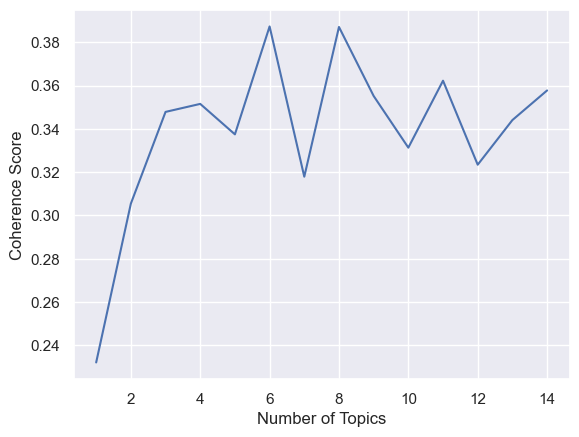
\includegraphics[width=\textwidth]{cv.png}
    \caption{Coherence for $c_v$ approach}
    \label{cv}
\end{subfigure}
\hfill
\begin{subfigure}{0.45\textwidth}
    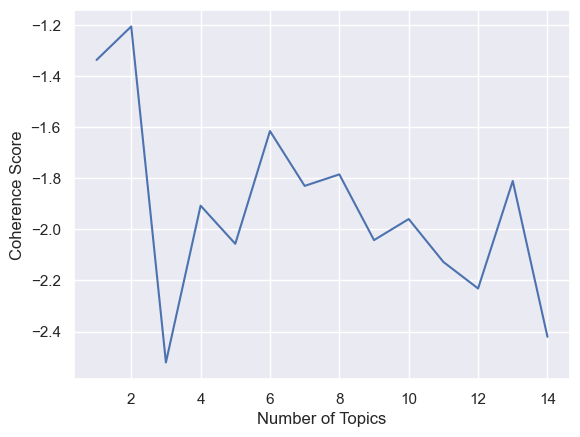
\includegraphics[width=\textwidth]{umass.png}
    \caption{Coherence for $u_{mass}$ approach}
    \label{umass}
\end{subfigure}       
\caption{Coherence score to estimate optimal number of Topics}
\label{cv_umass}
\end{figure}

From the chart we can see that six topics are dominant in our provided
corpus. The chart shown at the left shows the coherence score for
\(u_{mass}\) and the right chart represents the score for \(c_{v}\) for
multiple iterations. Using 6 topics we can see the output of
corresponding topic and top 10 words in a topic.


\begin{longtable}[]{@{}
  >{\raggedright\arraybackslash}p{(\columnwidth - 4\tabcolsep) * \real{0.17}}     
  >{\raggedright\arraybackslash}p{(\columnwidth - 4\tabcolsep) * \real{0.83}}@{}}
\toprule
Topics & Dominant Keywords and Weights \\
\midrule
\endhead
\textbf{Topic 01} & \enquote*{energy} 0.060, \enquote*{source} 0.029, \enquote*{renewable} 0.018, \enquote*{water}0.016, \enquote*{use} 0.013, \enquote*{gas} 0.013, \enquote*{produce} 0.013, \enquote*{green} 0.013, \enquote*{warm}
0.013, \enquote*{cause} 0.012 
\\
\textbf{Topic 02} & \enquote*{pastime} 0.024, \enquote*{computer} 0.024, \enquote*{social} 0.023, \enquote*{user} 0.022, \enquote*{network} 0.020, \enquote*{student} 0.019, \enquote*{class} 0.017, \enquote*{change} 0.016, \enquote*{book} 0.015, \enquote*{survey} 0.013  
\\
\textbf{Topic 03 }& \enquote*{mother} 0.083, \enquote*{buy} 0.021, \enquote*{love} 0.018, \enquote*{child} 0.014, \enquote*{worker} 0.014, \enquote*{begin} 0.013, \enquote*{cultural} 0.012, \enquote*{observe} 0.012, \enquote*{thing} 0.012, \enquote*{language} 0.011 
\\ 
\textbf{Topic 04} &  \enquote*{life} 0.016, \enquote*{Bangladesh} 0.016, \enquote*{family} 0.015, \enquote*{home} 0.014, \enquote*{root} 0.014, \enquote*{language} 0.014, \enquote*{country} 0.013, \enquote*{Pakistan} 0.010, \enquote*{war} 0.010, \enquote*{man} 0.009 
\\ 
\textbf{Topic 05} & \enquote*{country} 0.031, \enquote*{river} 0.022, \enquote*{India} 0.022, \enquote*{land} 0.021, \enquote*{boat} 0.015, \enquote*{small} 0.015, \enquote*{population} 0.015, \enquote*{lake} 0.013, \enquote*{group} 0.012, \enquote*{house} 0.011 
\\ 
\textbf{Topic 06} & \enquote*{job} 0.064, \enquote*{English} 0.023, \enquote*{learn} 0.021, \enquote*{teacher} 0.017, \enquote*{use} 0.016, \enquote*{dream} 0.016, \enquote*{think} 0.016, \enquote*{thing} 0.015, \enquote*{school} 0.014, \enquote*{education} 0.013\\
\bottomrule
\end{longtable}




%\textbf{Topic 01}: {[}\enquote*{energy} 0.060, \enquote*{source} 0.029, \enquote*{renewable} 0.018, \enquote*{water}
%0.016, \enquote*{use} 0.013, \enquote*{gas} 0.013, \enquote*{produce} 0.013, \enquote*{green} 0.013, \enquote*{warm}
%0.013, \enquote*{cause} 0.012,{]}

%\textbf{Topic 02}: {[}\enquote*{pastime} 0.024, \enquote*{computer} 0.024, \enquote*{social} 0.023, \enquote*{user}
%0.022, \enquote*{network} 0.020, \enquote*{student} 0.019, \enquote*{class} 0.017, \enquote*{change} 0.016,
%\enquote*{book} 0.015, \enquote*{survey} 0.013,{]}

%\textbf{Topic 03}: {[}\enquote*{mother} 0.083, \enquote*{buy} 0.021, \enquote*{love} 0.018, \enquote*{child} 0.014,
%\enquote*{worker} 0.014, \enquote*{begin} 0.013, \enquote*{cultural} 0.012, \enquote*{observe} 0.012,
%\enquote*{thing} 0.012, \enquote*{language} 0.011,{]}

%\textbf{Topic 04}: {[}\enquote*{life} 0.016, \enquote*{Bangladesh} 0.016, \enquote*{family} 0.015, \enquote*{home}
%0.014, \enquote*{root} 0.014, \enquote*{language} 0.014, \enquote*{country} 0.013, \enquote*{Pakistan}
%0.010, \enquote*{war} 0.010, \enquote*{man} 0.009,{]}

%\textbf{Topic 05}: {[}\enquote*{country} 0.031, \enquote*{river} 0.022, \enquote*{India} 0.022, \enquote*{land} 0.021,
%\enquote*{boat} 0.015, \enquote*{small} 0.015, \enquote*{population} 0.015, \enquote*{lake} 0.013, \enquote*{group}
%0.012, \enquote*{house} 0.011,{]}

%\textbf{Topic 06}: {[}\enquote*{job} 0.064, \enquote*{English} 0.023, \enquote*{learn} 0.021, \enquote*{teacher}
%0.017, \enquote*{use} 0.016, \enquote*{dream} 0.016, \enquote*{think} 0.016, \enquote*{thing} 0.015,
%\enquote*{school} 0.014, \enquote*{education} 0.013{]}

\subsection{Count vs Relative Importance measurement}

Word frequency $n(w_{j},d_{i})$ in each document \(D\) is measured as below which identifies the most frequent words within each document and across the entire corpus.

\begin{equation}
D = \sum_{d_{i} \in D}^{}\left\{ \begin{array}{l}
1,n\left( w_{i},d_{i} \right) > 0 \\
0,n\left( w_{i},d_{i} \right) = 0 \\
\end{array} \right.\
\end{equation}

we can visualize relative importance of any keywords in terms of frequency and plotted inclined with LDA provided weights.

\begin{figure}[h]
\centerline{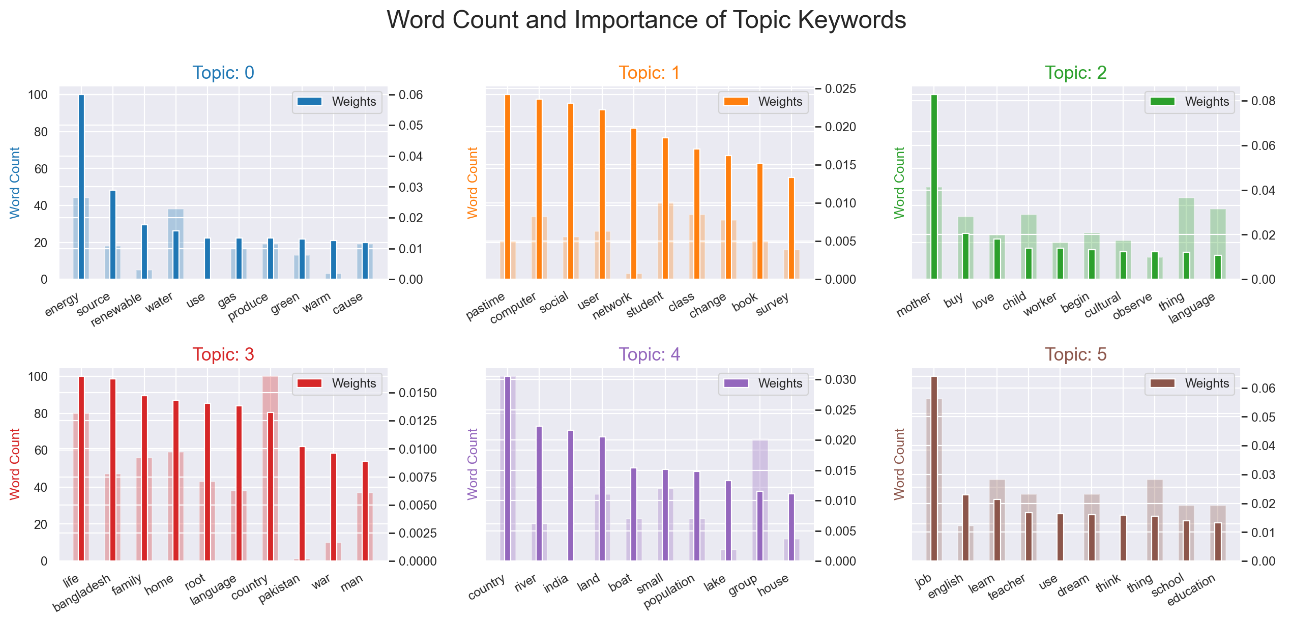
\includegraphics[width=\textwidth]{relative_imp.png}}
\caption{Word frequency and its relative importance}
\label{fig:Relative_weight}
\end{figure}

\section{Dominant topic and contribution}

In LDA models, each document is composed of multiple topics. But
typically, some specific topics are dominant. The following experiment
extracts this dominant topic for each sentence and shows the relative
weight of the topic and the keywords. It estimated which document
belongs predominantly to which topic. How frequently the words have
appeared in the documents and the weights of each keyword in the same
chart, words that occur in multiple topics and the ones whose relative
frequency is more than the weight.

\subsection{Topic-Term Matrix Visualization and Inter-Topic Distance Map}

Visualizing the topics and their relationships in a topic model Python
library PyLDAvis is used provides an interactive web-based interface to
explore and analyze the LDA results of topic modeling. PyLDAvis itself
abstracts away much of the underlying mathematical complexity and
provides a user-friendly way to generate visualizations and
interactively explore topics and their relationships. Key components
distance among topics and salient terms are explained below:

\subsubsection{Inter-Topic Distance Map}

Distance among topics refers to the measurement of similarity between
topics in a high dimensional space matrix provided by the LDA model.
PyLDAvis library is used to conserve dimensionality reduction using PCA
and for calculating distance between topics metric like Euclidean
distance or Cosine Similarity \(\). Topic-topic distribution matrix
\(Q\left( t_{1},t_{2} \right)\) for topic \(t_{1}\) and topic \(t_{2}\),
distance \(D\)between \(t_{1},t_{2}\) can be represented as

\subsubsection{Salient Terms or dominant keywords}

Salient Terms in a topic are words \(W\) that are most strongly
associated with specific topic. The mathematical expression for finding
salient terms \(w\) for a topic \(t\) involves, extraction of top
\(n\)words that poses the highest probability scores for topic \(t\) in
the topic-term matrix \(P\lbrack t,w\rbrack\).

\begin{figure}[h]
\centerline{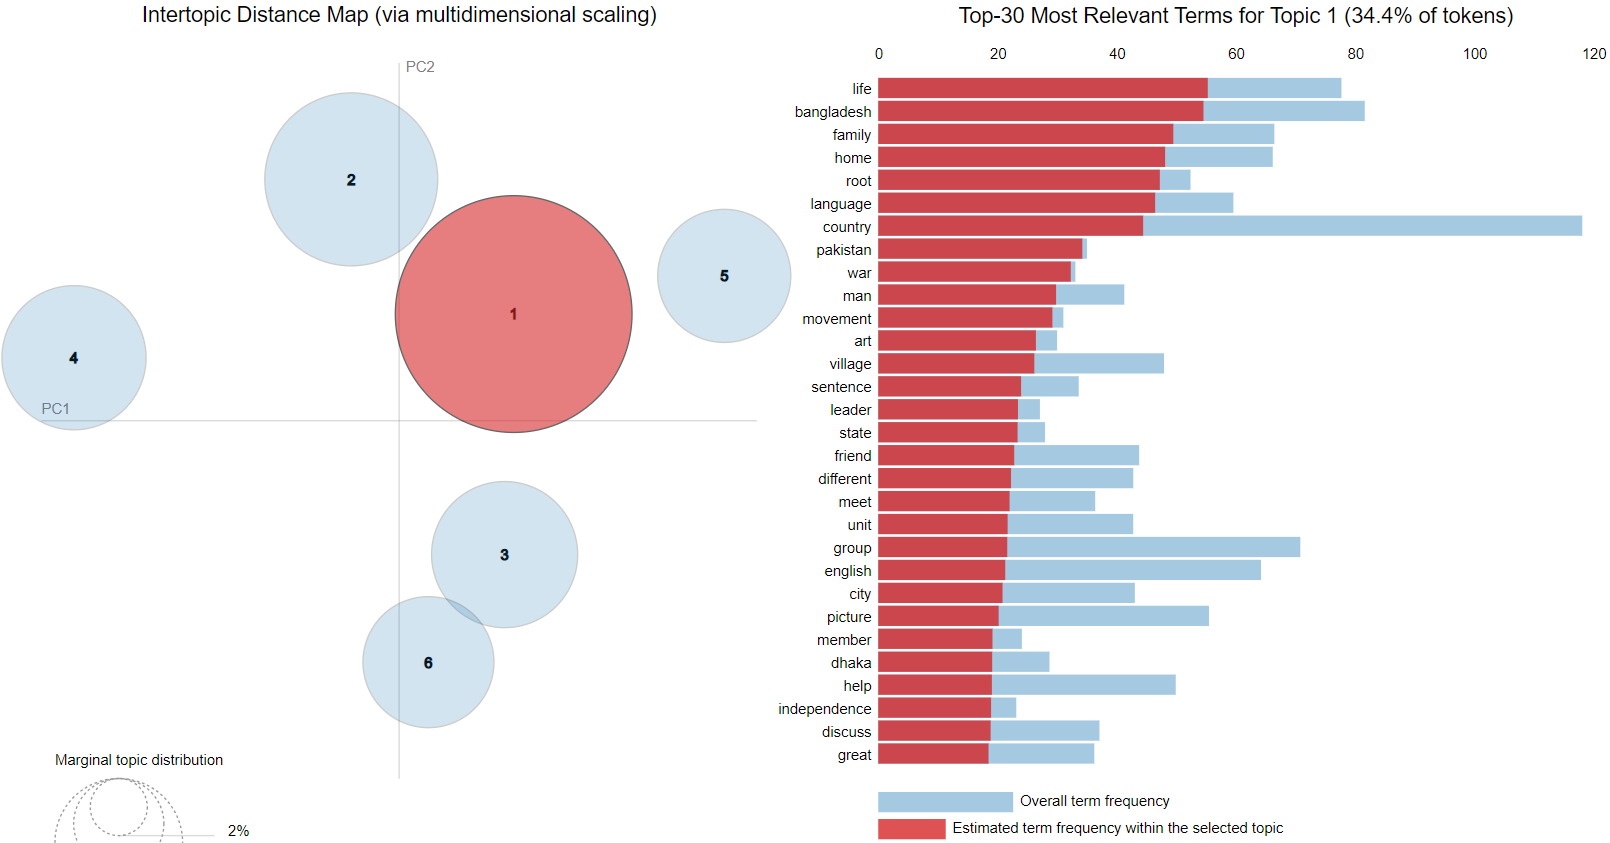
\includegraphics[width=\textwidth]{pyldvis.png}}
\caption{Topic model co-occurrence visualization with dominant keywords'}
\label{fig:Relative_weight}
\end{figure}

Top 30 most salient terms are showed at right in the bar chart histogram
and left figure shows inter topic distance, their size etc. PCA
dimensionality reduction technique is applied here to embed the LDA
result into a 2D plain scale. Projected the data in lower-dimensional
subspace by computing eigenvalues reduced the circle overlapping. Topics
that are closer together in the map are more similar in terms of the
distribution of words.

\section{Englisher Mobile App}
A mobile application (Englisher) is being developed with content from the NCTB’s English Textbook for class 9. The extracted keywords are organized into lessons and furthermore quiz is introduced as an exercise. Each sentence's and word's Bengali meaning is provided in accordance with the lesson. Students can take quizzes, and their results are recorded in the history so that history can be reviewed and performance can be improved by more practice in the future. 

\begin{figure}[h!]
\centering
\begin{subfigure}{\textwidth}
	\centering
    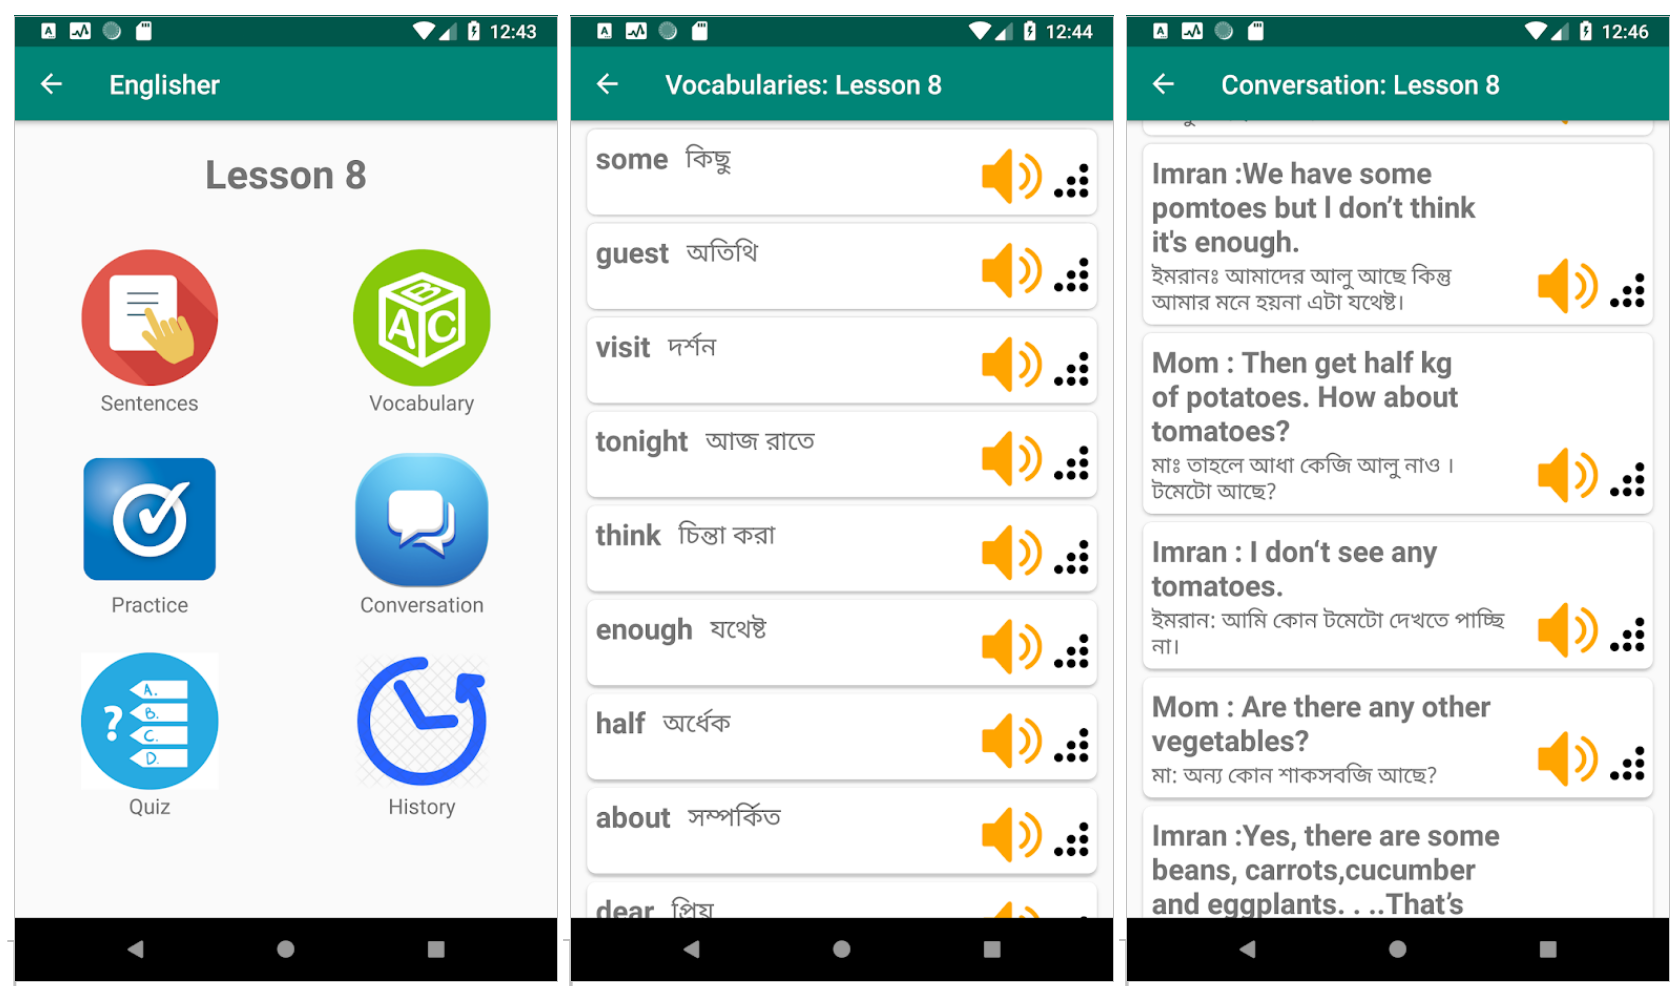
\includegraphics[width=\textwidth]{mobile_app_01.png}
    \caption{Lesson wise exercise}
    \label{fig:first}
\end{subfigure}
\hfill
\begin{subfigure}{\textwidth}
	\centering
    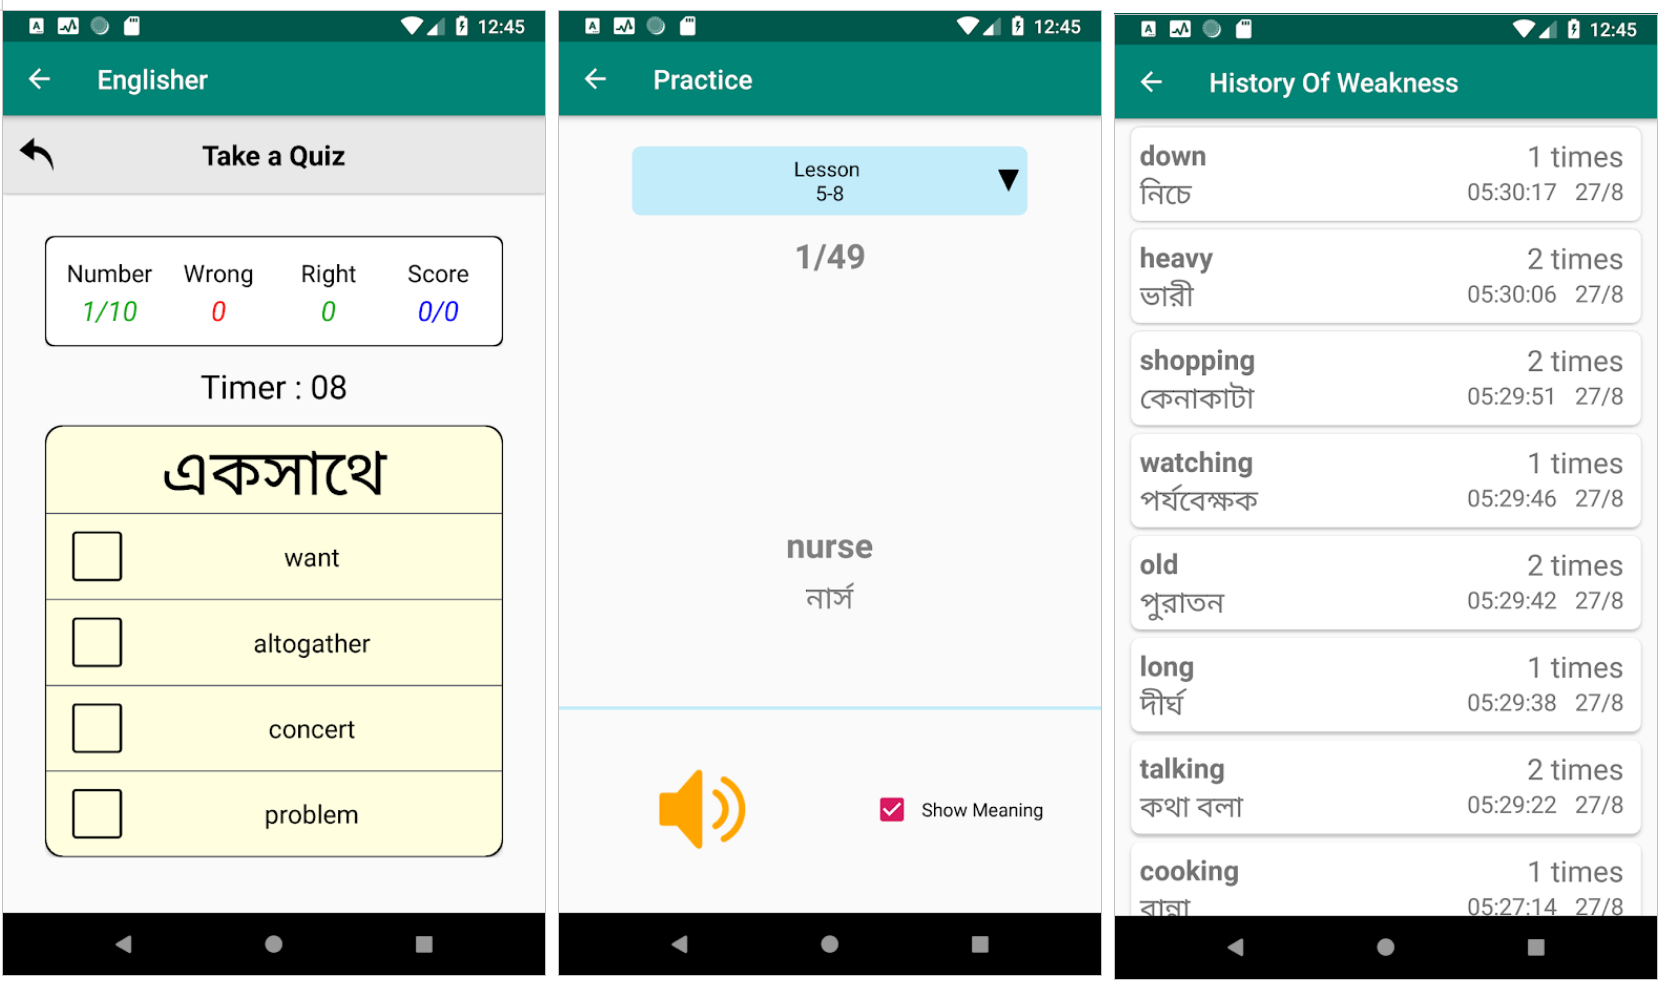
\includegraphics[width=\textwidth]{mobile_app_02.png}
    \caption{Quiz with Vocabulary}
    \label{fig:second}
\end{subfigure}
        
\caption{Englisher Mobile app for Learning LDA based topic model words}
\label{fig:figures}
\end{figure}

\section{Qualitative survey}
In the survey questions, it was indicated whether the students, teachers/instructors, and government organizations would find it acceptable and appreciated if textbook information were made available through a mobile app and presented in interactive format. To demonstrate the mobile app idea during the interrogation survey session prototype app Englisher is prepared. Participants were asked for suggestions on how to make the app better and specify shortcomings. Presumably It provides an insight of teacher’s emotion about inclusion of mobile technology in higher secondary English education system. 

\subsection{Survey Planning}
The survey was conducted over a period of four weeks, with 50 High schools in Dhaka and Bogura district of Bangladesh. It encompasses only English subject areas Teachers who teaches in high schools from class six to class Ten and teaches regularly in the school. A questionnaire was distributed to teachers allowing us to gather questionnaire answer. 
\subsubsection{Survey participants}
During the survey standard participants were chosen emphasizing infrastructure quality, teaching experience, class size etc. At the beginning from 100 institution were selected. Then half of them were excluded since those institutions infrastructure's overall quality and condition were not above average. Among the chosen samples 76\% were good and 26\% considered average institutions. Privately held 45\%, 32\% partially government and 22\% are government institutes.  Over 1000 students study in almost 40\% of these institutions and  sizable number of pupils are present in each section and class. 38\% class have a size greater than 50. So, we can presume that the participating teachers have quite a bit of experience teaching sufficient number of students.  
\subsection{Survey Results}
We have done extensive analysis with the survey data collected. In our data collection highest priority is given for the secondary class student teachers who teach between 6-10th class about 46\%. High school, KG college and KG High school. Details about the statistics are depicted in the following figure. Adjacent chart explains the percentage of teachers who teach in which class. Hence, from these two figures we can get a vivid image of collected dataset resources about the participating teachers. 

\begin{figure}[h!]
\centering
\begin{subfigure}{0.48\textwidth}
    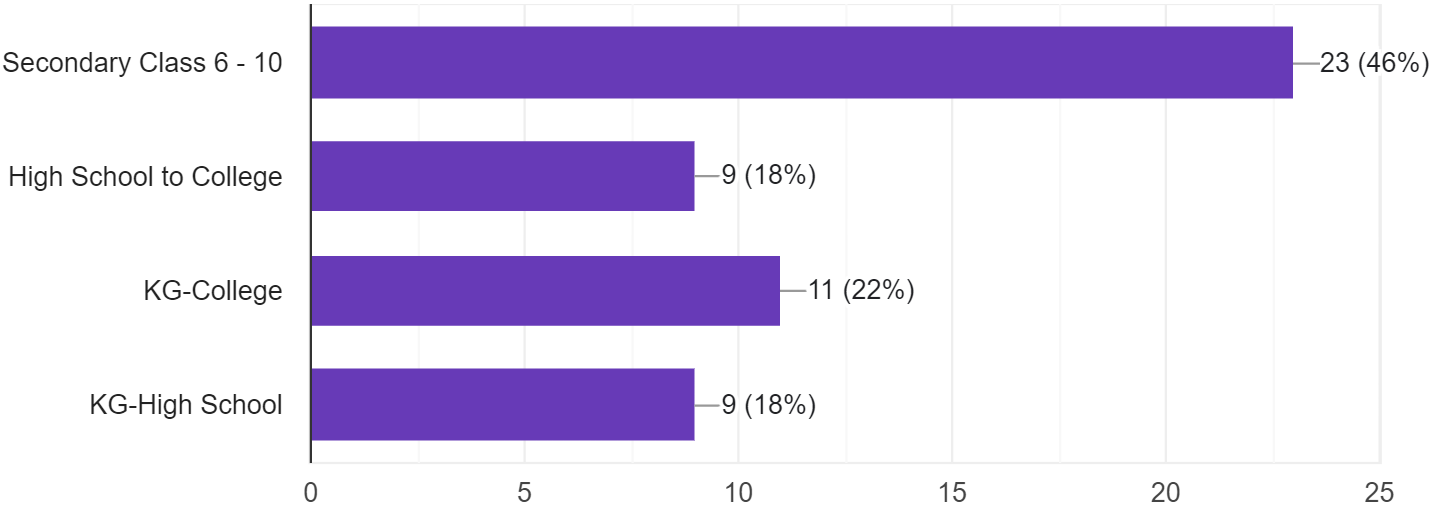
\includegraphics[width=\textwidth]{institution_size.png}
    \caption{Participating institution category and size}
    \label{cv}
\end{subfigure}
\hfill
\begin{subfigure}{0.48\textwidth}
    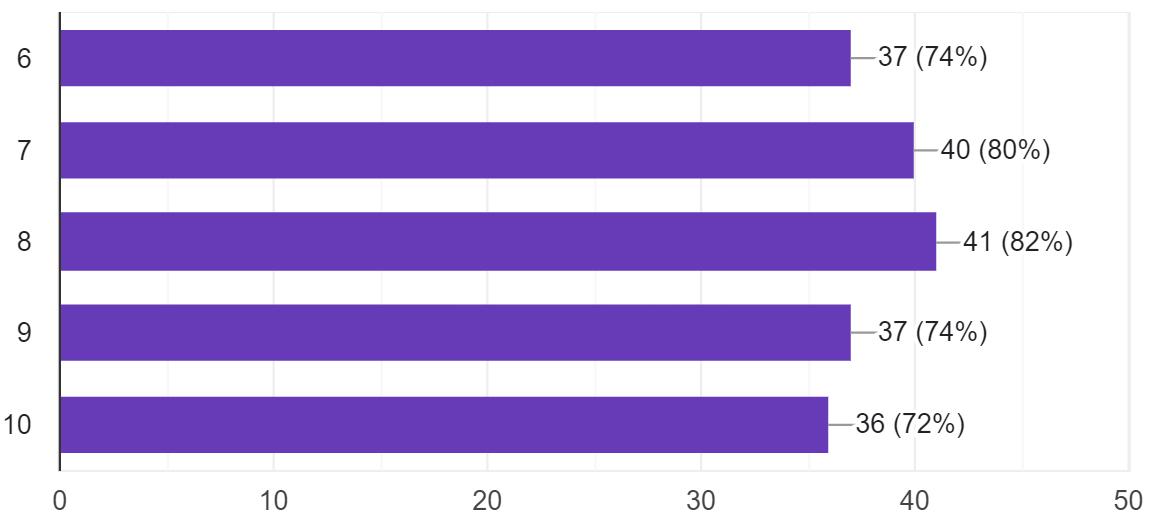
\includegraphics[width=\textwidth]{english_teaching_class.png}
    \caption{Participating instructors' class/Label}
    \label{umass}
\end{subfigure}       
%\caption{Coherence score to estimate optimal number of Topics}
\label{cv_umass}
\end{figure}

The following graphs give an overview of the English teaching experiences of the teachers as well as the general consensus regarding the use of digital content and mobile apps in everyday teaching and learning. Almost 62\% of teachers have been teaching for more than 8 to 10 years, and some of them have been teaching for decades in higher secondary education. 32\% of teachers have three to eight years of experience, while just 6\% are fresh to the profession. Around 83.7\% of teachers the language of instruction during their graduation was English, and their major was also English. Very few teachers 13.3\% graduation major is something other than English yet teaching English in secondary schools probably have sufficient English language proficiency.  

\begin{figure}[h!]
\centering
\begin{subfigure}{0.48\textwidth}
    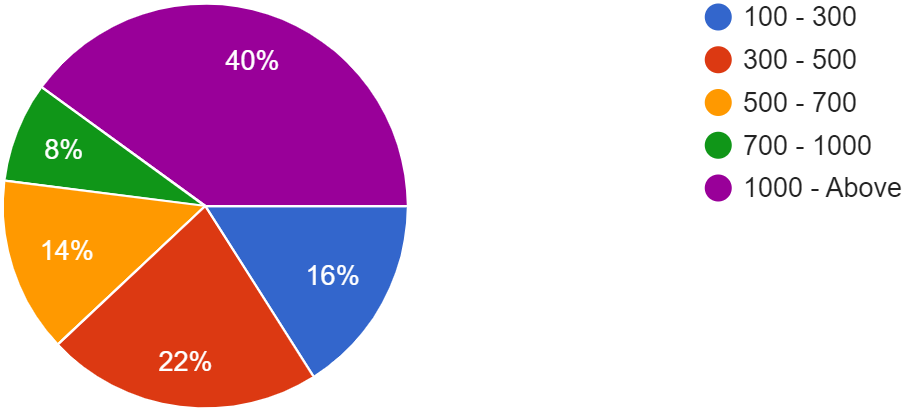
\includegraphics[width=\textwidth]{num_stu.png}
    \caption{Participating institutions' number of students}
    \label{cv}
\end{subfigure}
\hfill
\begin{subfigure}{0.48\textwidth}
    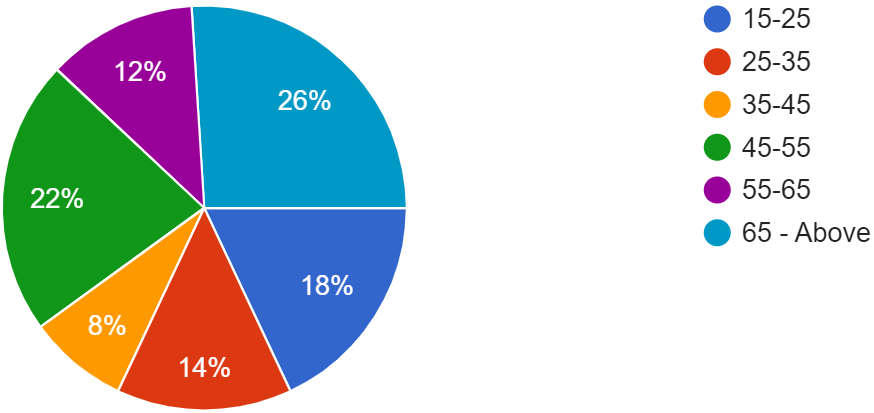
\includegraphics[width=\textwidth]{class_size.png}
    \caption{Participating instructors' class size}
    \label{umass}
\end{subfigure}       
%\caption{Coherence score to estimate optimal number of Topics}
\label{cv_umass}
\end{figure}

\subsubsection{Analyzing survey Facts} 
More than half of teachers, or 58\%, have no prior experience utilizing mobile apps or technology for teaching, but 90\% of them agree, and more than 45\% strongly agree, that it encourages pupils to engage actively in their learning. However, they (almost 60\%) also hold the opinion that a notebook cannot be completely replaced, despite the fact that mobile apps may solve many problems and provide technological support for teaching and learning. Promisingly optimistic approximately 40\%, although thinking that the notebook-based content memorizing learning method can be replaced, feel that mobile app-based learning can replace it permanently. 

\begin{figure}[h!]
\centering
\begin{subfigure}{0.48\textwidth}
    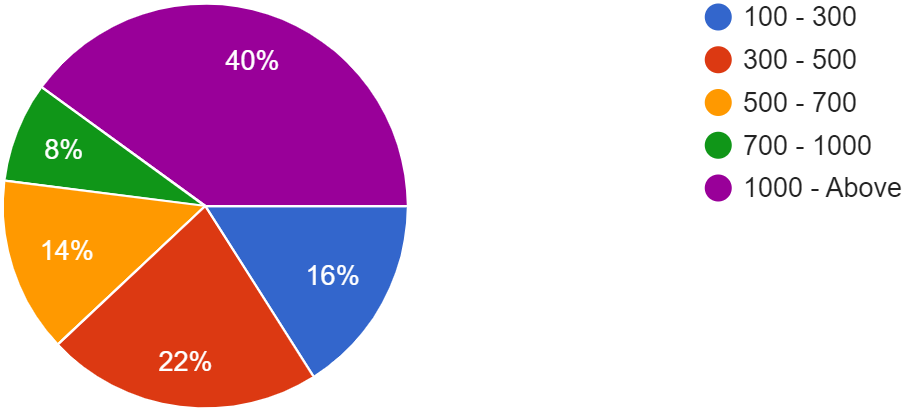
\includegraphics[width=\textwidth]{num_stu.png}
    \caption{Participating institutions' number of students}
    \label{cv}
\end{subfigure}
\hfill
\begin{subfigure}{0.45\textwidth}
    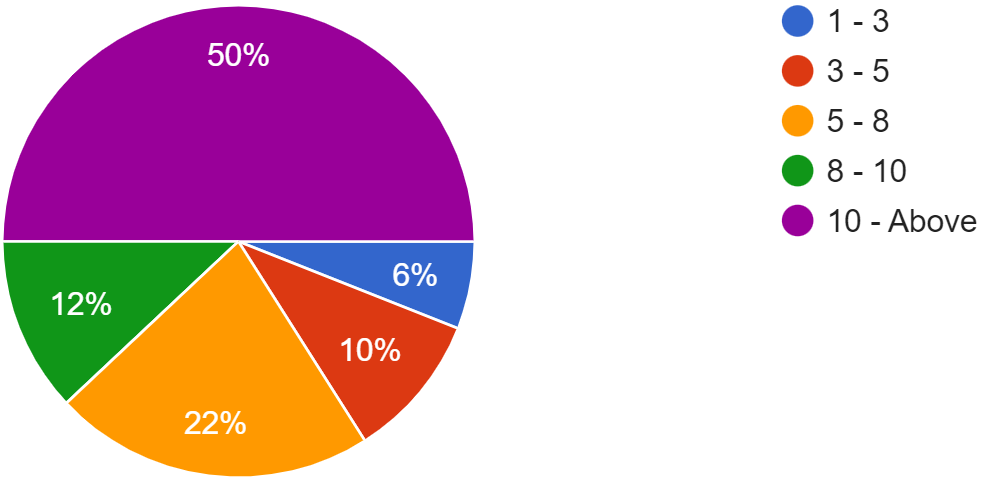
\includegraphics[width=\textwidth]{experience.png}
    \caption{Participating instructors' Teaching experience}
    \label{umass}
\end{subfigure} 
\begin{subfigure}{0.44\textwidth}
    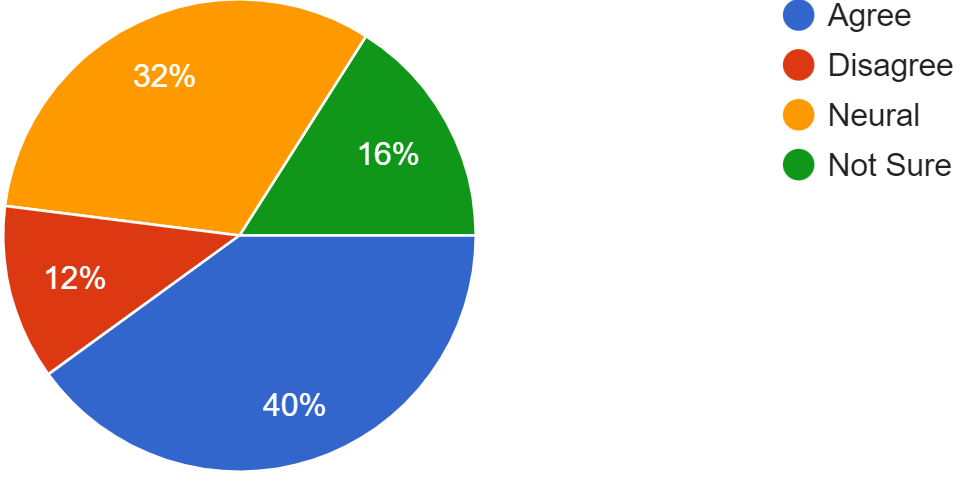
\includegraphics[width=\textwidth]{replace.png}
    \caption{App could help students in replacement of guide book}
    \label{cv}
\end{subfigure}
\hfill
\begin{subfigure}{0.47\textwidth}
    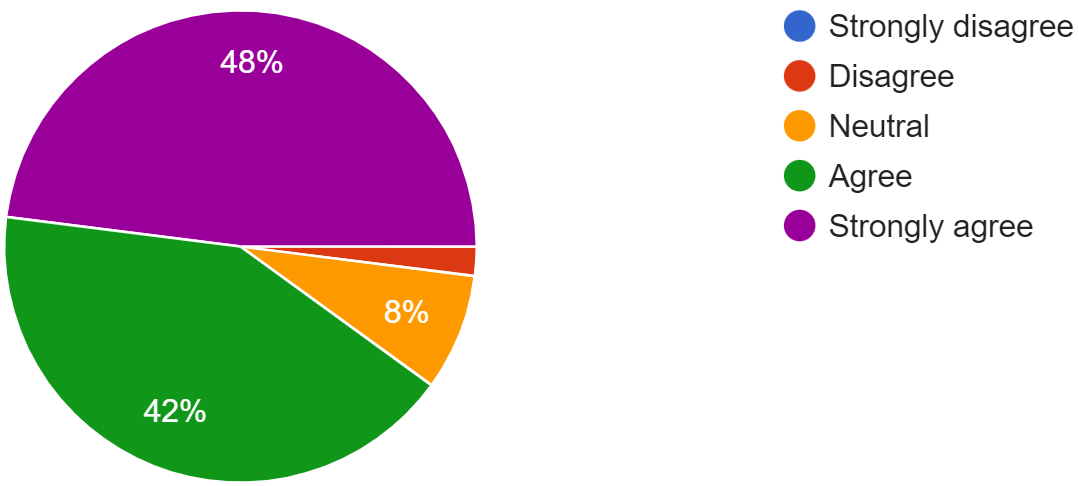
\includegraphics[width=\textwidth]{app_motivates.png}
    \caption{App could motivate students}
    \label{umass}
\end{subfigure}        
%\caption{Coherence score to estimate optimal number of Topics}
\label{cv_umass}
\end{figure}

This study proposes the Englisher mobile app and presents it to the participating teachers to gather their insightful feedback. 92\% of teachers reported that they would use this type of mobile app for teaching if it were made available after using the trial version of the offered customized Englisher app. Teachers anticipate that 80\% of students will utilize this app during class. 86\% of respondents believed it may help students' English proficiency, and 98\% agreed that the government should support this kind of innovation in the education sector. 

\begin{longtable}[]{@{}
  >{\raggedright\arraybackslash}p{(\columnwidth - 4\tabcolsep) * \real{0.7732}}
  >{\raggedright\arraybackslash}p{(\columnwidth - 4\tabcolsep) * \real{0.1066}}
  >{\raggedright\arraybackslash}p{(\columnwidth - 4\tabcolsep) * \real{0.1203}}@{}}
\toprule
\begin{minipage}[b]{\linewidth}\raggedright
\textbf{Questions}
\end{minipage} & \begin{minipage}[b]{\linewidth}\raggedright
\textbf{yes}
\end{minipage} & \begin{minipage}[b]{\linewidth}\raggedright
\textbf{No}
\end{minipage} \\
\midrule
\endhead
Do you use digital content for teaching or digital medium for teaching
and learning & 84\% & 16\% \\
Have you ever used Internet or Mobile app to teach students or asked
students to find learning materials from internet or Mobile App & 76\% &
24\% \\
Education during graduation was English and English was used for
learning & 83.70\% & 16.30\% \\
\multicolumn{3}{@{}>{\raggedright\arraybackslash}p{(\columnwidth - 4\tabcolsep) * \real{1.0000} + 4\tabcolsep}@{}}{%
\textit{Customized mobile app for Learning and Teaching English}} \\
Do you think teacher will use the topic model mobile app for teaching &
92\% & 8\% \\
Do you think students will use the topic model app for learning? & 80\%
& 20\% \\
Do you think topic model based mobile app-based learning can improve
English proficiency of students & 86\% & 14\% \\
Do you think Govt should promote these types of innovation for education
sector & 98\% & 2\% \\
\bottomrule
\end{longtable}


\section{Linguistic Inquiry and Word Count (LIWC) for Qualitative sentiment}
\label{liwc}

In this research LIWC is used to ascertain the general sentiment of the
responses given by the survey participants. Linguistic Inquiry and Word
Count (LIWC), is a text analysis tool to measure
psychological or emotional characteristics \cite{tausczik2010psychological, liwc22_welcome_nodate}. It aims to quantify
sentiment by examining the frequencies of different linguistic terms
within given text based on predefined dictionary of words associated
with various categories. Let's assume text as a sequence of words:
\(\left\{ w_{1},w_{2},\ldots.,w_{n} \right\}\) and M different
linguistic categories: \(\left\{ C_{1},C_{2},\ldots.,C_{m} \right\}\) .
Proportion of words in each category
\(P\lbrack i\rbrack = \frac{w\lbrack i\rbrack}{T}\) where T is the total
number of Text. Now, a matrix \(X\lbrack i,j\rbrack\) can be formed,
where \(w_{i}\) represents the frequency of the word in the linguistic
category \(C_{j}\). LIWC vector containing the proportions of words in
each linguistic category can be expressed as
\(P_{total}\lbrack j\rbrack = \frac{\sum_{i = 1}^{T}{X\lbrack i,j\rbrack}}{T}\).

\begin{longtable}[]{@{}
  >{\raggedright\arraybackslash}p{(\columnwidth - 12\tabcolsep) * \real{0.1709}}
  >{\raggedright\arraybackslash}p{(\columnwidth - 12\tabcolsep) * \real{0.1042}}
  >{\raggedright\arraybackslash}p{(\columnwidth - 12\tabcolsep) * \real{0.1794}}
  >{\raggedright\arraybackslash}p{(\columnwidth - 12\tabcolsep) * \real{0.1045}}
  >{\raggedright\arraybackslash}p{(\columnwidth - 12\tabcolsep) * \real{0.1756}}
  >{\raggedright\arraybackslash}p{(\columnwidth - 12\tabcolsep) * \real{0.1016}}
  >{\raggedright\arraybackslash}p{(\columnwidth - 12\tabcolsep) * \real{0.1638}}@{}}
\toprule
\begin{minipage}[b]{\linewidth}\raggedright
\textbf{Traditional LIWC Dimension}
\end{minipage} & \begin{minipage}[b]{\linewidth}\raggedright
\textbf{Answer Text}
\end{minipage} & \begin{minipage}[b]{\linewidth}\raggedright
\textbf{Standard Commercial Language}
\end{minipage} & \begin{minipage}[b]{\linewidth}\raggedright
\textbf{Answer Text}
\end{minipage} & \begin{minipage}[b]{\linewidth}\raggedright
\textbf{Standard for Formal Language}
\end{minipage} & \begin{minipage}[b]{\linewidth}\raggedright
\textbf{Answer Text}
\end{minipage} & \begin{minipage}[b]{\linewidth}\raggedright
\textbf{Standard for story language}
\end{minipage} \\
\midrule
\endhead
\textbf{Positive Tone} & 2.54 & 3.96 & 3.91 & 2.33 & 3.22 & 2.18 \\
\textbf{Negative Tone} & 0 & 1.1 & 0 & 1.38 & 0 & 1.75 \\
\textbf{Social Words} & 2.54 & 6.87 & 5.65 & 6.54 & 4.08 & 10.5 \\
\textbf{Cognitive Processes} & 13.56 & 9.35 & 18.26 & 7.95 & 15.88 &
8.7 \\
\textbf{Allure} & 2.54 & 7.79 & 3.04 & 3.58 & 2.79 & 5.48 \\
\textbf{Moralization} & 0 & 0.2 & 0 & 0.3 & 0 & 0.21 \\
\bottomrule
\end{longtable}

From this LIWC table higher proportion of words related to positive
emotions indicate a positive emotional tone in the text in the answer
for the questions related to ``How this app can be improved'' and ``How
English learning can be improved using Mobile App''. LIWC is applied for
three different categories ``commercial writing'', ``Formal language'',
and ``story language'' and in all the categories answer text showed
highly positive sentiment from the survey user. Though respondents had a
mix of optimism and skepticism regarding the use of mobile apps in
teaching and learning. During the interrogation session, their tone was
positive and enticed participants.

\subsection{Visualize participants response with Word cloud}
\label{wordcloud}
LIWC involves linguistic analysis using mathematical expression but
using word cloud survey answers can be visualized vividly in
interpretable interactive format. Word cloud consider a set of words
\(\left\{ w_{1},w_{2},\ldots.,w_{n} \right\}\) extracted from Text
document and associated frequencies
\(\left\{ f_{1},f_{2},\ldots.,f_{n} \right\}\), \(s_{i}\) represent the
proportional size of the word in the cloud can be expressed as
\(s_{i} = \frac{f_{i}}{\sum_{j = 1}^{n}f_{j}}\) where normalized
frequency \(f_{i}\).

\begin{figure}[h!]
\centering
\begin{subfigure}{0.48\textwidth}
    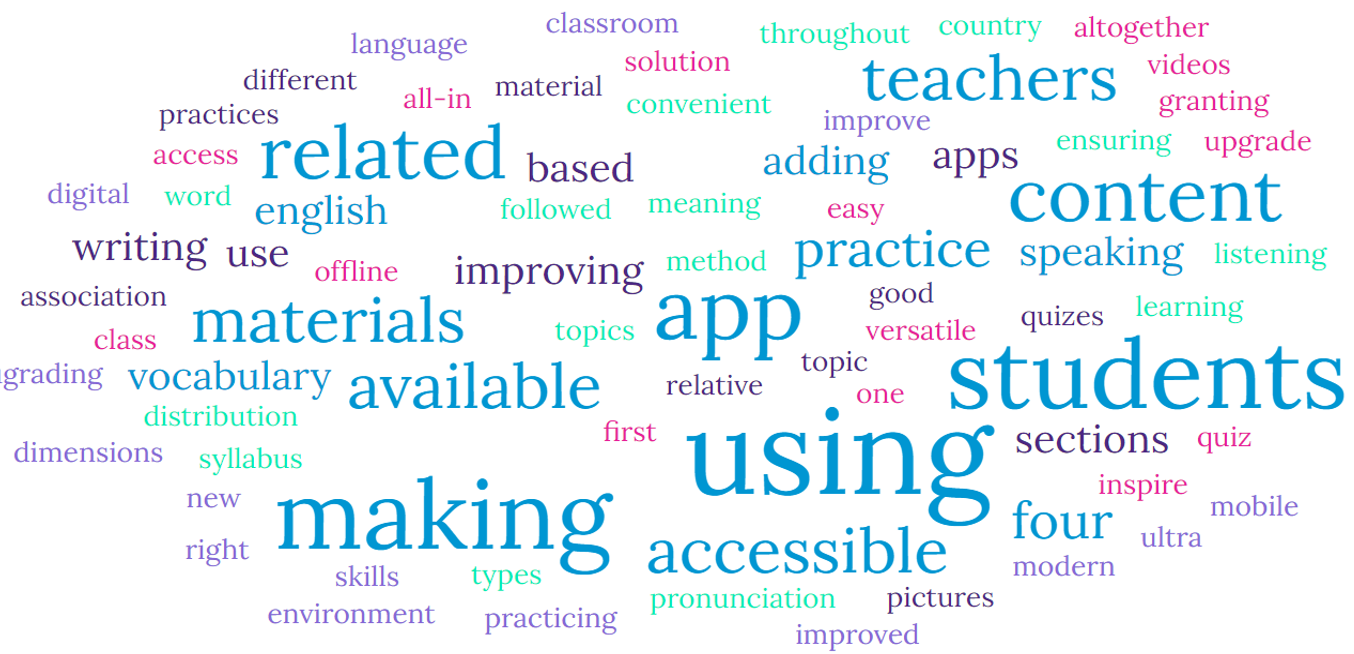
\includegraphics[width=\textwidth]{app_impv.png}
    \caption{word cloud for the question regarding app improvement}
    \label{cv}
\end{subfigure}
\hfill
\begin{subfigure}{0.48\textwidth}
    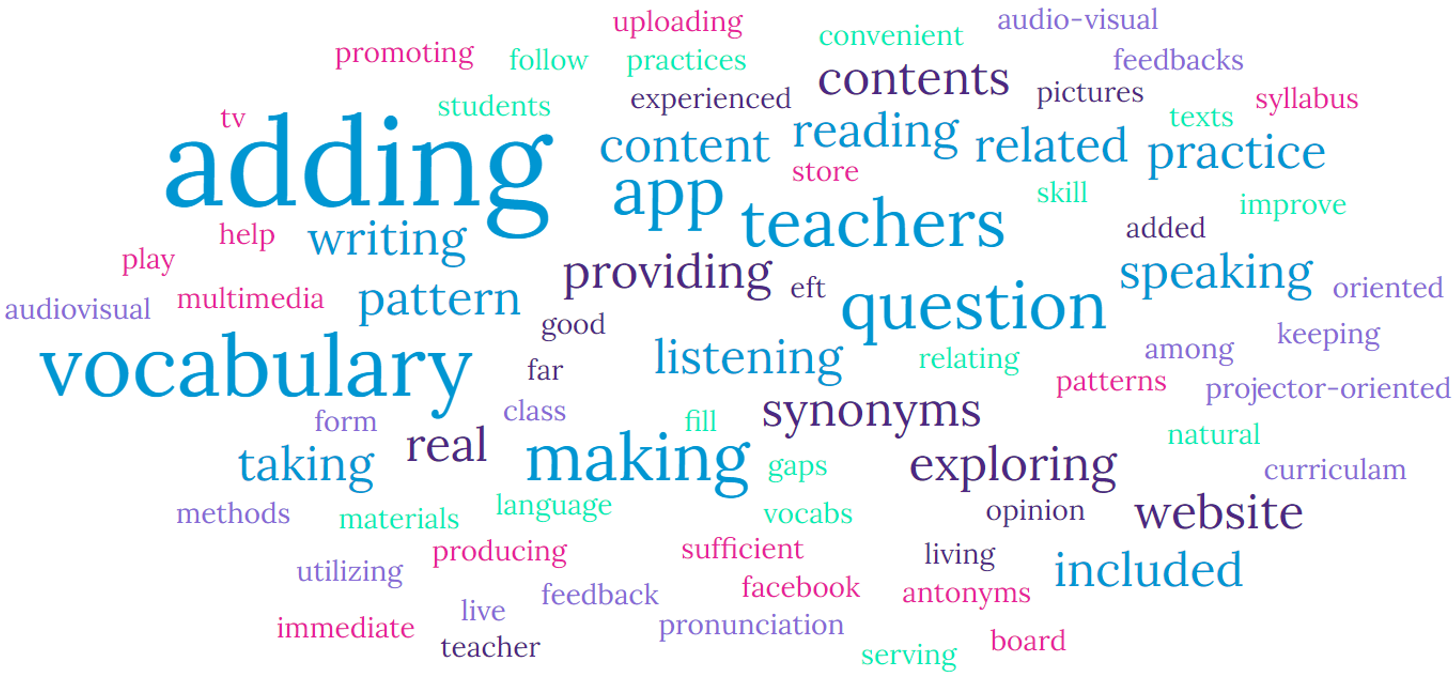
\includegraphics[width=\textwidth]{eng_app_impv.png}
    \caption{word cloud for the question regarding English learning app improvement}
    \label{umass}
\end{subfigure}       
%\caption{Coherence score to estimate optimal number of Topics}
\label{cv_umass}
\end{figure}

The word cloud is generated from the answers provided question ``how the
app can be improved'' and followed by more generalized question ``how
English learning can be improved using an App''. The participants
narrated varieties of viewpoints for the questions. From the word cloud
it is inferred adding graphical content would enhance the
apps\textquotesingle{} usefulness and make them more visually appealing
to users. More practice resources for listening and exercise would be
helpful. Another suggestion is to include synonym, and syllabus-related
instances as well as audiovisual engagement with the app. Add additional
vocabulary and involve more experience teachers who have greater
experience in digital learning and teaching.

\section{Results Discussion and outcomes}

The results demonstrate that LDA-based topic modeling significantly
enhances content comprehension by providing concise summaries of the
learning material. Readers can grasp the main ideas and connections
between topics, aiding in retention and knowledge acquisition. From the
qualitative survey it is revealed LDA based topic modeling approach
based extracted keywords within mobile apps seem effective as it
provides more contextual meaning to the learners. Most of the
participating teachers are enthusiastic about topic modeling based
contexual resources learning related to technology incorporating into
pedagogy. Participants appreciated the cutting edge NLP's learning
resources available through mobile devices. Teachers admitted that
available digital resources facilitated a deeper understanding of topics
and catered to different learning styles, nurturing more engaging
learning environment. This will positively impacted student motivation
and overall engagement and hence boost overall learning. Some crucial
suggestions were improving the graphics of the app so that it becomes
interactive and guardian involvement can be introduced. Based on the
survey results, it is revealed the potential for digital mobile-based
learning in school is immense. Government should take initiatives to
incorporate it into course curriculum syllabus and could impose
ordinance to adopt mobile app based learning teaching in the school.

Apps need to be improved by including collaborative form of learning.
Additionally, the interactive interface receives positive feedback for
its user-friendly design and utility in assisting
readers\textquotesingle{} navigation through the textbook.
Recommendation is to make it specific for NCTB Books only for particular
class. This approach is also our goal considering NCTB Books. Including
interactive e-books, dictionary, educational apps, and multimedia
content.

\section{Limitations}

LDA could play a role in understanding the topics covered in an English
textbook and potentially aiding in content customization and topic
relevance for personalized learning. In a personalized learning context,
the goal is to tailor the educational experience to the individual needs
and preferences of each learner. This involves understanding the
learner\textquotesingle s strengths, weaknesses, interests, and learning
style. While LDA could be useful in some aspects of this process, it
might not directly address all the requirements of personalized learning
for an English textbook. In this research study we showed that LDA based
topic modeling could be a solution to enhance the context understanding
of the learners. However from the survey it is revealed that app was not
sufficient. Learners oriented topic-document distribution to identify
which topics are most relevant to a specific student can be provided.
App can provide additional explanations, examples, or resources to cater
to their individual learning style. Assessments and exercises focused on
the topics that need reinforcement for each student. Monitor their
progress and adjust the learning path accordingly. Analyze
students\textquotesingle{} performance, engagement, and feedback to
refine the topic modeling process and its integration into the learning
environment. More sophisticated approaches, such as adaptive learning
systems and AI-based tutoring, might be needed to truly personalize the
learning experience in a comprehensive manner.

\section{Special Remarks}

For the data privacy and security issues many Teachers were reluctant to
provide their social website address to the surveyor. Among all the
participants only 24\% attendees provided their social sites address to
use them publicly for research purposes.

\section{Conclusion}
By employing topic modeling in a personalized learning context,
educators can create more engaging and effective learning experience.
This approach allows enhancement understanding and retention of the
Textbook context. The school survey with prototype app reaffirmed its
potential in learning experiences. LDA based topic modeling leverages
learning experience, improve interpretation and knowledge acquisition.
The synthesis of existing research sheds light on the potential of topic
modeling to improve Textbook context comprehension, and knowledge
retention of learners. It was revealed teachers/instructors would find
it acceptable and appreciated if textbook information were presented
using NLP technology driven algorithms like LDA topic modeling in mobile
app. The study concludes apps seem effective as they provide a personal
and learner-centered learning opportunity ubiquitously. Reveal to user
as a complementary essential material to learn English Textbook quickly
and effectively. However, apps need to be improved by including
collaborative form of learning.

\subsection{Training Dataset}
In this research we have used dataset from \cite{gaur2019knowledge}. For training classifier in this research 2019's Gaur et. al \cite{gaur2019knowledge} dataset is used. Compared to the existing four-label classification scheme (no risk, low risk, moderate risk, and high risk), this dataset introduced 5 lavel classification suicide indicator, ideation, behavior, attempt and another extra category incorporating supportive category. Supportive category represents whenever someone shows empathy and condolence for a suicidal post. 

\subsection{Testing/Validation Dataset} 
For testing dataset is collected from kaggle. It is an opesource dataset publicly available collected from reddit website by a pushshift API contained suicide and depression category.  This publicly available Reddit datasets in Kaggle Website comprised of 232,074 post annotated for binary classification as suicidal or non-suicidal in \cite{aldhyani2022detecting} for detecting suicidal ideation. The dataset is a collection of posts from the "SuicideWatch" and "depression" subreddits of the Reddit platform. All posts that were made to "SuicideWatch" from Dec 16, 2008(creation) till Jan 2, 2021, were collected while "depression" posts were collected from Jan 1, 2009, to Jan 2, 2021. In this research trained classifier is applied to detect class on this two category. Main objective isto determine the suicide categories (indicator, ideation, behavior, attempt, supportive ) within this dataset. Document length frequency and token distribution is depicted in Figure \ref{redditdist}. From the frequency distribution we can see some of the document sizes are very large. Hence, during the training process we chopped the sentences into multiple sentences keeping the label same. 

\subsection{Data Processing and Models}
\subsubsection{Data Pre-processing}\label{data_preprocessing}
Social media dataset are mostly Text data which needs data pre-processing, cleaning, feature extraction and data mining related NLP tasks. NLP based text data contains noises such as: unnecessary quotes, special characters, punctuation etc. Moreover, morphological analysis is needed to retrieve root words followed by stemming, lemmatization. Then, sentences are divided into equal-length fragments, and null word padding is applied as needed. Words within a phrase are now referred to as tokens or features, and the dataset is shown as a corpus. Special features/tokens are further preprocessed and filtered using text data feature extraction tools and methods. Features are passed through a process in which features are converted to corresponding IDs and sentences which contains a series of IDs are represented a vector. The embedding is another term that is frequently used in relation to vector text analysis. Various Vectorization methods are present. Traditional vectorization method provide weights to terms/words mainly based on frequency of words within the sentence and documents, rather than its importance and contextual meaning. Also, how does a particular word or term create impact on the neighboring words is not taken into consideration, since these models does not have any prior knowledge of any words. Hence, various neural network based language models are proposed which are pretrained on massive amount of dataset. These models mainly carries weight which represents word to word relationships and most cases can provide contextual meaning of given sentence based on pretrained dataset knowledge. Deep learning models recently showed remarkable achievements in this case representing corresponding knowledge.

\subsubsection{Classification}
Machine learning and Deep Learning models are particularly used for Text classification and ML for feature selection or extraction in several studies \cite{castillo2020suicide, chancellor2020methods, zhang2022natural}. These extensive reviews reveal Deep learning methods receive more attention and perform better than traditional machine learning methods whereas in some cases when extracted or filtered features are fit into training process models are able to perform better. NLP techniques are applied for the annotated dataset collected from Twitter, Reddit, Facebook, instagram, Weibo \cite{wang2020depression} etc. After that various deep learning and machine learning models are trained for classification of suicide and depression. Then trained models are applied to determine the correct class of given text. \cite{malhotra2022deep} Provided a through investigation about passed research techniques, features, datasets, and performance metrics \cite{zhang2022natural, chancellor2020methods}. 

\subsubsection{Data Learning Models}
Among Several Deep Learning approaches most successful NLP classifier for segregating Depression and suicidal task are CNN, LSTM, GRU, XLNET, BERT, Variants of BERT RoBERTa and variants of CNN such as: CNN-BiLSTM etc \cite{aldhyani2022detecting, wang2020depression, shetty2020predicting} also showed promising results. 

\subsubsection{Feature Selection} 
The feature selection procedure has a substantial impact on the performance of machine learning and deep learning models because it lowers noise in the trained dataset, enabling the model to accurately understand data patterns. LIWC, LDA, LSA, n-gram analysis \cite{pennebaker2001linguistic, tadesse2019detection} etc are used as features analysis tools. 
Most dominant approaches are n-gram word frequency based approach TF-IDF. Apart from the Deep learning model n-gram Traditional feature retrieve based analysis conducted in some research papers. In 2017 Shen et. al \cite{harvesting_social_media} collected several forms of features comprised of six chorots, namely, social network features, user profile features, visual features, emotional features, topic-level features, and domain-specific features and prepared a feature rich dictionary. This multimodal depressive dictionary learning model was used to detect the depressed users on Twitter using machine learning models. 

Most dominant approaches are Word2Vec, XGBoost, SVM, Random Forest, other regression MLs. Typical word embedding approaches TF-IDF and Word2Vec, and CNN–BiLSTM are applied in  \cite{aldhyani2022detecting}. Using LIWC features, XGBoost ML together surpasses the accuracy of CNN–BiLSTM in  \cite{aldhyani2022detecting}. Others have used machine text Summarization based feature extraction strategy followed by classification for depression detection is applied in \cite{zogan2021depressionnet}. \cite{burnap2015machine}built a set of baseline classifiers using lexical, structural, emotive and psychological features extracted from Twitter posts. Then baseline classifiers are updated by building an ensemble classifier using the Rotation Forest algorithm and a Maximum Probability voting classification decision method. \cite{chancellor2020methods} This paper provided an excellent overview of 75 studies in between 2013 and 2018 outlining the methods of data annotation for mental health status, data collection and quality management, pre-processing and feature selection, and model selection and verification. 

\subsection{Other Tools or Methods}
Apart from the Machine Learning or statistical model approaches there are some sites, helpline numbers and apps \cite{martinengo2019suicide} that contains various facts, statistics, tips, tools, healthline numbers and ways to handle suicidal depression \cite{suicidaldepression_online}. 
  
nce, visualizing the result we can determine the suicidal tendency within depression post. Also, N-gram based analysis is conducted and frequency of Terms and connections of words or phrases are analyzed in this research scope. More often topic modeling clustering is used to determine latent topic and understand latent text network. From the network various facts can be revealed related to suicide and depression. This whole process is depicted in Figure \ref{fig:res_diagram}


\section{Results Analysis}\label{sec2}
First we started our experiment with document length distribution. The length of document and term frequency within the corpus is visualized in Figure \ref{redditdist_twitterdist}. From the distribution we can see that some of the document length are excessive long and contains more than 1000 tokens ( within Twitter and also Reddit both Dataset). Depression class document length are usually shorter in length. Depression document length are tend to be smaller than suicide document length. 

Short sentence does not carry much terms and hence does not carry enough information to be classified confidently by classifier algorithms. We started reducing the numbers of samples based on document length. By reducing the samples based on numbers of tokens present in a document (see Figure \ref{redditdist_twitterdist}). Documents length versus category frequency information is showed in this chart. This charts explains if we filter out the shorter comments suicide post become dominant class and depression post become outnumbered. The difference showed an exponential pattern as length of document increases. Test dataset Reddit data distribution among depression and suicide class distribution ratio is equal. Filtering the class we have seen an interesting fact that depressed people does not want to comment very long. 



\subsection{N-gram Analysis}
\subsubsection{Uni-gram}
Dataset is split into separate tokens after preprocessing and uni-gram generated. Based on frequency of words wordcloud is generated from these unigrams. Frequency based comparison between two categories is conducted for depression and suicide for Test dataset in Figure \ref{features_vis_pro_exp}. Main objective was to get top ranked words from Depression and Suicide corpus. After experiments we have seen There are similarities between the top ranked words those are occurring frequently. They tend to use slang and abusive terms compared to suicidal attempt thinking people. Rather suicidal depressed people want to share their thoughts with others using longer post. However, it does not reveals any clues in terms of hypothetical relationships between the two category. It is difficult find pattern in which we can determine the depression and suicidal thought. So far we found some pattern 
%\begin{enumerate}
%\item short statements likely to be more depression category
%\item Depressive statements tend to have slang
%\item Suicidal thinking people’s post having very high frequency of “kill” “die” these type of words or phrases.
%\end{enumerate}
%
%\begin{figure}[H]
%\centering
%\begin{subfigure}{0.45\textwidth}
%    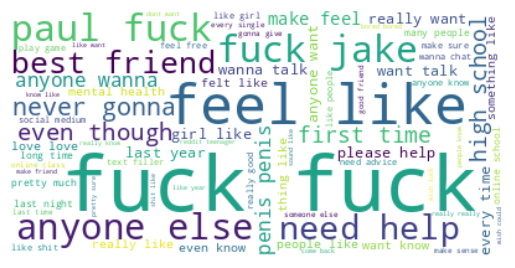
\includegraphics[width=\textwidth]{dep_wordcloud.png}
%    \caption{Wordcloud in Depression category}
%    \label{fig:first}
%\end{subfigure}
%\hfill
%\begin{subfigure}{0.45\textwidth}
%    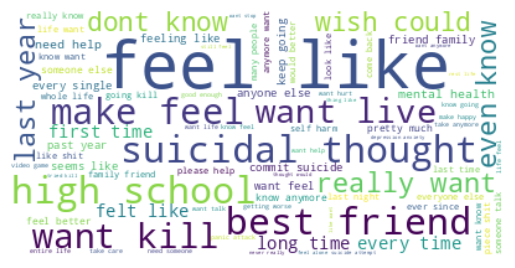
\includegraphics[width=\textwidth]{sui_wordcloud.png}
%    \caption{Wordcloud in Suicide category}
%    \label{fig:second}
%\end{subfigure}
%\hfill
%\begin{subfigure}{0.8\textwidth}
%    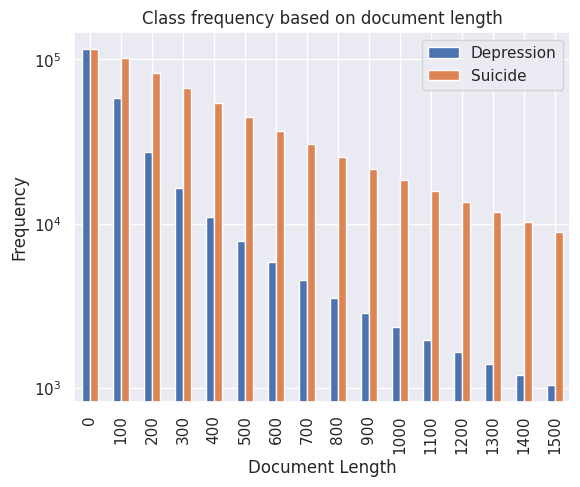
\includegraphics[height=7.5cm, width=\textwidth]{doc_len.png}
%    \caption{Class frequency in different Document Length}
%    \label{fig:second}
%\end{subfigure}        
%\caption{Dataset features visualization and properties exploration}
%\label{features_vis_pro_exp}
%\end{figure}

To understand the term occurring frequently in two different classes scatterplot library is used for visual analysis. From the above two scenario we can see that there is a pattern that people used to say more slang and abusive words when they are depressed. It is also interesting that there are many words have high frequency such as depression or depressed but belongs to suicide class. One important fact is revealed here is that we can see although suicide, suicidal these words has high frequency in Suicide class but depression, depressed also occurred in parallel with high frequency. Here several experiments can be conducted for exploratory analysis with scattertext library for terms significance. However, this library is computationally heavy for larger dataset for visualization. Another drawbacks is this library have significant focus on the terms based analysis. We have used simple vectorization methods by which we can have greater control on dataset and experiments code. 

\subsubsection{Bi-gram}
First unigram is computed and analyzed then bigram is calculated for both categories. The bigram frequency showed there are some common terms like “mental health”, “feel like”, “make feel”, “high school” etc showed high occurrences in the dataset. Hence, we started to understand its pattern in the corpus. For analysis we have considered ['high school', 'mental health', 'best friend', 'feel like', 'really want', 'suicide thought', 'friend family'] these bi-grams and wanted to explore its surrounding context for each category. We called this special bigrams since it showed importance in the suicidal and depression both categories appeared highly frequent matter. We want to analyze how these words have impact with its neighboring words. 

To explore the impact of special bi-grams on the samples, special bi-gram terms containing samples are filtered from dataset. After that using lebel encoder bigrams are encoded as integers and then chord diagram is generated  depicted in Figure \ref{Bigram_features_exp} to find meaningful relationship within the samples between the bigram features.  


%\begin{figure}[H]
%\centering
%\begin{subfigure}{0.8\textwidth}
%    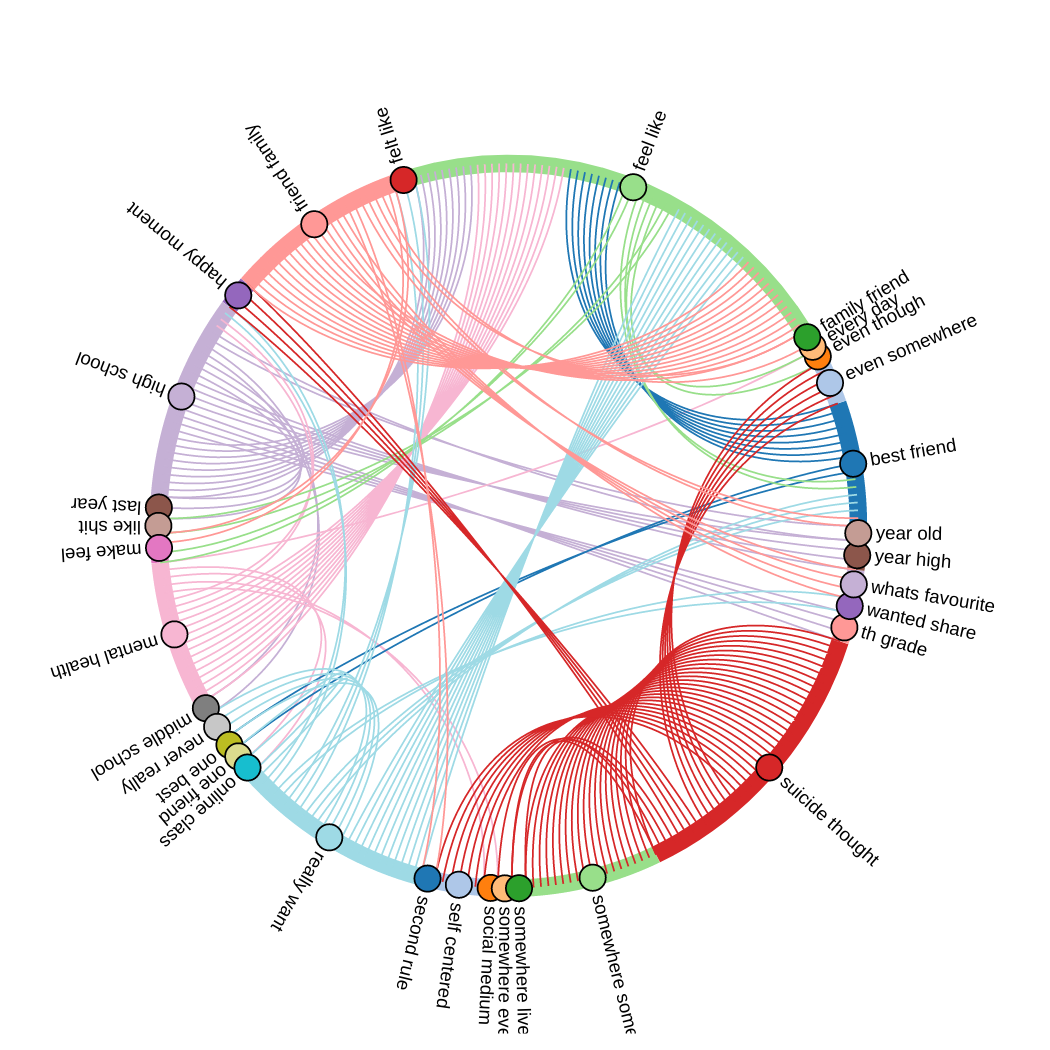
\includegraphics[width=\textwidth]{dep_chord.png}
%    \caption{Depression Chord diagram}
%    \label{fig:first}
%\end{subfigure}
%\hfill
%\begin{subfigure}{0.8\textwidth}
%    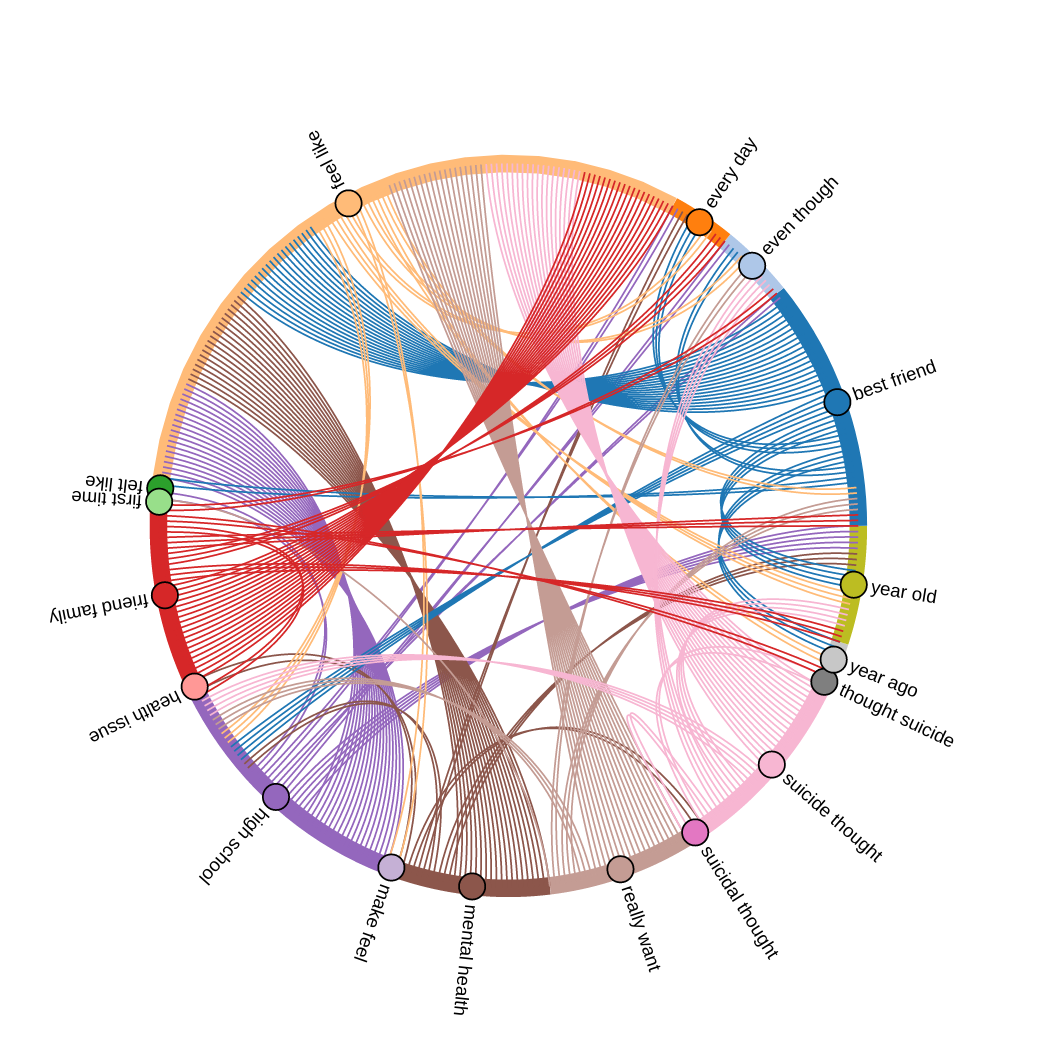
\includegraphics[width=\textwidth]{suicide_chord.png}
%    \caption{Depression Chord diagram}
%    \label{fig:second}
%\end{subfigure}        
%\caption{Bi-gram features relation exploration}
%\label{Bigram_features_exp}
%\end{figure}


From this two chord diagram interesting sentence can be inferred. Such as: from the depression class ? self centered person is depressed, having suicidal thought, want to go somewhere to live, spend happy moments and so on. For the suicidal class category suicidal attempt thinking people, have mental health issue, they want to share though with high school friends, best friends, friends and family members, having suicidal thoughts and so on.  

Tri-grams or above did not reveals much meaning information, mostly does convey some meaningful information and therefore excluded for further experimental consideration. 

\section{Classification Results}
To segregate the Reddit suicide dataset into different categories of suicide first we have created a classifier using different classification techniques. Since our objective is not making highly accurate classifier. Following approach is applied in this study

\begin{itemize}
\item Pre-processed and useful features are used from Twitter's 500 post CSSR dataset for Training classifier
\item Used count vectorizer and TFIDF transformer to generate vectors for the dataset
\item Trained classifier to determine the categories of various suicidal intensities
\end{itemize}

We have used simple gridsearch technique of sklearn library and from a list of various classifiers applied on the dataset, we have chosen highest accurate classifiers to determine different label of suicidal risk. so that it can recognize the category. We have used classifiers "K Nearest Neighbors", "Linear and RBF SVM", "Gaussian Process", "Decision Tree", "Random Forest", "Vanilla Neural Net", "AdaBoost", "Naive Bayes". Using various set of parameters, from the result and experiments we found almost 60\% accuracy for SVM model to predict the suicide intensity categories. From various set of values of SVM we found degree=2, gamma=0.7, kernel=rbf showed the highest accuracy. 


%\begin{table}[h]
%\begin{center}
%\begin{minipage}{174pt}
%\caption{Caption text}\label{tab1}%
%\begin{tabular}{@{}lllll@{}}
%\toprule
%Classifier & Precision & Recall & Accuracy & F1 \\
%\midrule
%Nearest Neighbors & 0.926 & 0.924 & 92.3896 & 0.924\\
%RBF SVM & 0.942 & 0.924 & 92.3896 & 0.927\\
%Decision Tree & 0.901 & 0.848 & 84.7793 & 0.856\\
%Random Forest & 0.513 & 0.282 & 28.1583 & 0.167\\
%Neural Net & 0.942 & 0.927 & 92.6941 & 0.929\\
%AdaBoost & 0.905 & 0.898 & 89.8021 & 0.899\\
%Gaussian Process & 0.940 & 0.921 & 92.0852 & 0.924\\
%Naive Bayes & 0.923 & 0.918 & 91.7808 & 0.919\\
%QDA & 0.931 & 0.909 & 90.8676 & 0.912\\
%\botrule
%\end{tabular}
%\footnotetext{Shows classifiers accuracy of classification models}
%\end{minipage}
%\end{center}
%\end{table}

\subsubsection{Suicidal Intensities visualization}
How much depression can trigger suicidal thoughts is an interesting question. In this study classifier is trained on the suicidal intensity. Then trained classifier is applied on the Depression/Suicide class dataset. From various machine learning models we have found SVM is a good performing model. SVM classifier is applied for the TFIDF vectorizer embedding (see results in figure~\ref{SVMTFIDF}) and also for Word2vec pretrained vectorizer model. The results are shown in figure~\ref{Suicidal_int_vis}. From the results we can see that suicidal ideation between depression and suicidal categories number of samples are very similar. Within depression more number of samples are showed suicidal indicator category compared to suicide which is an interesting result. Suicidal behavior and attempt is comparatively high within the suicidal category than depression. Hence, figure~\ref{SVMTFIDF} result seems to be pretty obvious, except for suicidal ideation category. Also for the suicidal indicator symptoms are higher within the depression category. 

%\begin{figure}[H]
%\centering
%\begin{subfigure}{0.45\textwidth}
%    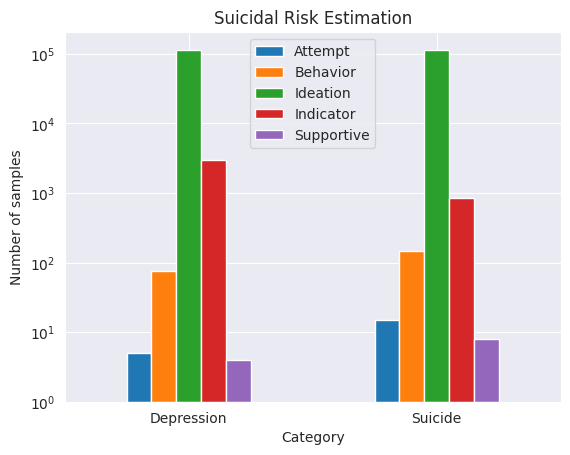
\includegraphics[width=\textwidth]{grid_svm.png}
%    \caption{SVM classifier applied for TFIDF vectorizer}
%    \label{SVMTFIDF}
%\end{subfigure}
%\hfill
%\begin{subfigure}{0.45\textwidth}
%    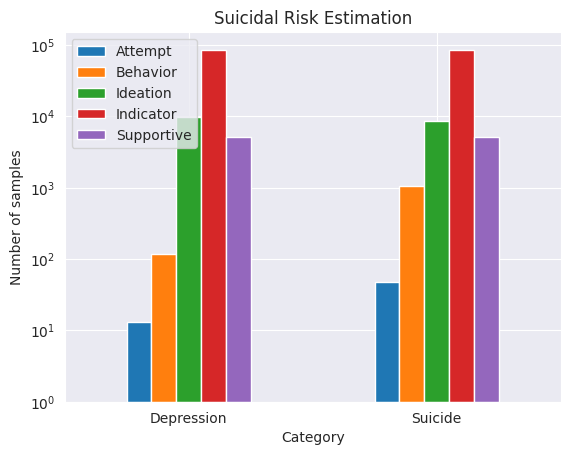
\includegraphics[width=\textwidth]{glove_vec.png}
%    \caption{SVM classifier applied for Glove Word2Vec Pretrained model vectorizer}
%    \label{GloveWord2Vec}
%\end{subfigure}        
%\caption{Visualizing suicide intensities within Depression/Suicide class}
%\label{Suicidal_int_vis} 
%\end{figure}

For the word2vec vector embedding scenario supportive and indicator categories results are almost similar in depression or suicide both classes. There is slight difference is shown for suicidal ideation and within suicide class, suicidal ideation is slight higher. Except the behavior and attempt category for the rest categories depression and suicide showed almost similar number of samples. 

%\begin{figure}[H]
%\centering
%\begin{subfigure}{0.45\textwidth}
%    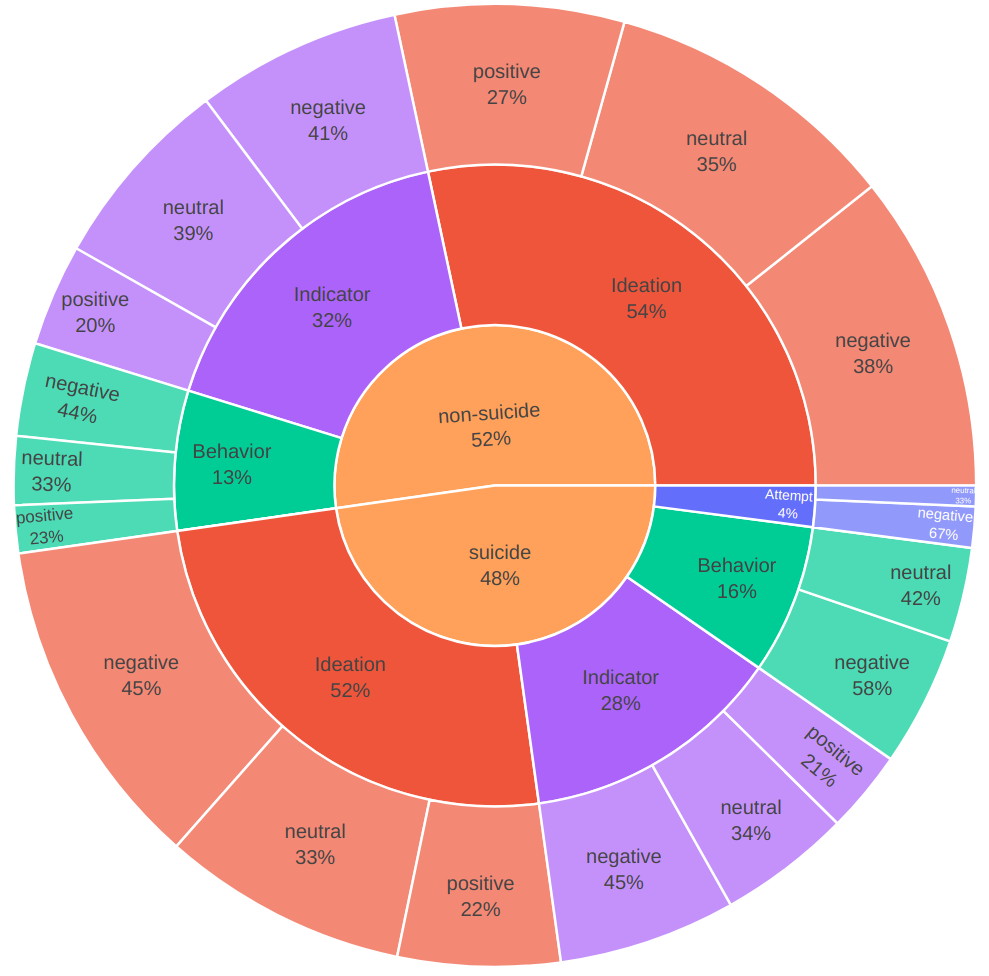
\includegraphics[width=\textwidth]{sentiment_sunburst.png}
%    \caption{First subfigure.}
%    \label{fig:first}
%\end{subfigure}
%\hfill
%\begin{subfigure}{0.45\textwidth}
%    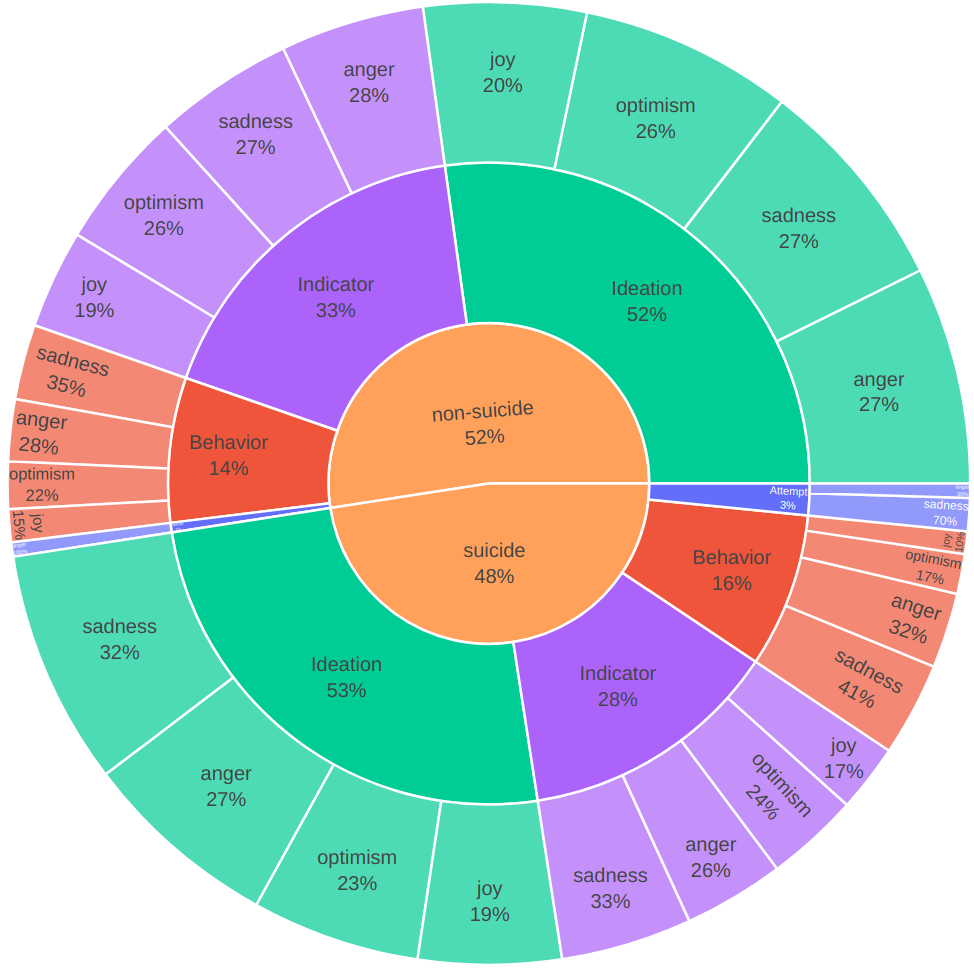
\includegraphics[width=\textwidth]{emotion_sunburst.png}
%    \caption{Second subfigure.}
%    \label{fig:second}
%\end{subfigure}
%        
%\caption{Subreferences in \LaTeX.}
%\label{fig:figures}
%\end{figure}
\section{Discussion} 
From the result it is revealed that suicide categories shown within depression and suicide class vividly. Specially suicidal ideation, indicator showed similar patterns. The number of samples within depression and suicide is almost similar for this two categories. Hence, we can infer depressed person comments showed suicidal ideation and suicidal indicating symptoms. Suicidal behavior and attempt showed higher number of samples within the suicide category compared to depression category. All these results seems very logical results. Although from the results mathematical formulas are not derived in this research study since results are susceptible to chosen classifier, chosen dataset, pretrained models vectors or embedding provided to the classifier. 
 
\section{Conclusion}
Suicidal risk estimation task and classification samples to determine suicidal risk within social websites and blogs, techniques are discussed before. According to suicidal category previous work has been done before. However, to what extent depression level triggers suicidal risk is not yet discussed before. Also it is difficult to determine since depression and suicide categorical variables are independent factor. There is not any underlying correlation. Several research conducted to segregate which post is suicidal and which one is depression various classifiers are proposed. Extensive work has been done to improve the classification accuracy by adopting most powerful vectorization techniques that uses cutting edge NLP models BERT and its various variants. Research has also been conducted on how much severity label of suicide within a post is studied. 

\bibliographystyle{plain} % We choose the "plain" reference style
\bibliography{Language_learning} % Entries are in the refs.bib file
\end{document}
